\chapter{Materials and methods}\label{chap:MatlsMethds}
To test if sewage sludge biochar effectively sorbs PFAS from PFAS-contaminated water and soil, a series of laboratory experiments with sorption isotherms were conducted. The aim of the experiments were to get a detailed mechanistic understanding of the sorption processes that occur when PFAS-contaminated water and soil are amended with waste biochar. Therefore, all experiments were prepared by spiking water with single PFASs and a cocktail of PFCA homologues. Six perfluorinated carboxylic acids with PFC-units 4-9 (PFPeA, PFHxA, PFHpA, PFOA, PFNA, PFDA) supplied by Merck Sigma-Aldrich were selected for the experiments conducted for this thesis. See \cref{tab:PFCAs} for a list of all native PFCAs including their respective CAS numbers and compound full names included in this thesis.  

The main work and laboratory experiments were conducted in the environmental chemistry laboratory at NGI, Oslo\footnote{Sognsveien 72, 0806, Oslo}. The quantification analysis was performed by UPLC-MS/MS at the Institute for Chemistry of Norwegian University of Science and Technology (NTNU), Trondheim\footnote{7491 Trondheim}. Biochar property characterization were performed at University of Florida, Gainsville\footnote{FL 32611, USA}. Iron and copper speciation was determined by XAS at the ESRF synchrotron. 

\begin{table}
\centering
\caption{Perfluorinated carboxylate acids (PFCAs) used in the sorption isotherm experiments. PFCs correspond to the number of perfluorinated carbon units in the chain. Note: PFCAs appear in dissociated form due to low $K_a$'s at environmentally relevant pH's. Supplied by Sigma Aldrich.}
\adjustbox{max width=\textwidth}{
\label{tab:PFCAs}
\begin{tabular}{@{}lcccclc@{}}
\toprule
\multicolumn{1}{c}{Chemical} & Acronym & Short & CAS number & Molecular structure & Stock form & Purity \\ \midrule
& & & & & &\\
\smash{\raisebox{4ex}{Perfluoropentanoic acid}}  & \smash{\raisebox{4ex}{PFPeA}} & \smash{\raisebox{4ex}{C5}} & \smash{\raisebox{4ex}{2706-90-3}} & \chemfig[atom style={scale=0.4}]{O=[:90](-[:30,,,1]OH)-[:150](-[:112.5]F)(-[:67.5]F)-[:210](-[:292.5]F)(-[:247.5]F)-[:150](-[:112.5]F)(-[:67.5]F)-[:210](-[:270]F)(-[:150]F)-[:210]F} & \smash{\raisebox{4ex}{liquid}} & \smash{\raisebox{4ex}{\textgreater 97 \%}} \\
& & & & & &\\
\smash{\raisebox{4ex}{Perfluorohexanoic acid}} & \smash{\raisebox{4ex}{PFHxA}}  & \smash{\raisebox{4ex}{C6}} & \smash{\raisebox{4ex}{307-24-4}} & \chemfig[atom style={scale=0.4}]{O=[:90](-[:30,,,1]OH)-[:150](-[:112.5]F)(-[:67.5]F)-[:210](-[:292.5]F)(-[:247.5]F)-[:150](-[:112.5]F)(-[:67.5]F)-[:210](-[:292.5]F)(-[:247.5]F)-[:150](-[:210]F)(-[:150]F)-[:90]F} & \smash{\raisebox{4ex}{liquid}} & \smash{\raisebox{4ex}{\textgreater 97 \%}} \\
& & & & & &\\
\smash{\raisebox{4ex}{Perfluoroheptanoic acid}} & \smash{\raisebox{4ex}{PFHpA}} & \smash{\raisebox{4ex}{C7}} & \smash{\raisebox{4ex}{375-85-9}} & \chemfig[atom style={scale=0.4}]{O=[:90](-[:30,,,1]OH)-[:150](-[:67.5]F)(-[:112.5]F)-[:210](-[:247.5]F)(-[:292.5]F)-[:150](-[:67.5]F)(-[:112.5]F)-[:210](-[:247.5]F)(-[:292.5]F)-[:150](-[:67.5]F)(-[:112.5]F)-[:210](-[:150]F)(-[:210]F)-[:270]F} & \smash{\raisebox{4ex}{crystalline}} & \smash{\raisebox{4ex}{\textgreater 99 \%}} \\
& & & & & &\\
\smash{\raisebox{4ex}{Perfluorooctanoic acid}} & \smash{\raisebox{4ex}{PFOA}}  & \smash{\raisebox{4ex}{C8}} & \smash{\raisebox{4ex}{335-76-2}}  & \chemfig[atom style={scale=0.4}]{O=[:90](-[:30,,,1]OH)-[:150](-[:67.5]F)(-[:112.5]F)-[:210](-[:247.5]F)(-[:292.5]F)-[:150](-[:67.5]F)(-[:112.5]F)-[:210](-[:247.5]F)(-[:292.5]F)-[:150](-[:67.5]F)(-[:112.5]F)-[:210](-[:247.5]F)(-[:292.5]F)-[:150](-[:90]F)(-[:150]F)-[:210]F} & \smash{\raisebox{4ex}{powder}} & \smash{\raisebox{4ex}{\textgreater 95 \%}} \\
& & & & & &\\
\smash{\raisebox{4ex}{Perfluorononaoic acid}}  & \smash{\raisebox{4ex}{PFNA}} & \smash{\raisebox{4ex}{C9}} & \smash{\raisebox{4ex}{375-95-1}} & \chemfig[atom style={scale=0.4}]{O=[:90](-[:30,,,1]OH)-[:150](-[:112.5]F)(-[:67.5]F)-[:210](-[:292.5]F)(-[:247.5]F)-[:150](-[:112.5]F)(-[:67.5]F)-[:210](-[:292.5])(-[:247.5]F)-[:150](-[:112.5]F)(-[:67.5]F)-[:210](-[:292.5]F)(-[:247.5]F)-[:150](-[:112.5]F)(-[:67.5]F)-[:210](-[:270]F)(-[:210]F)-[:150]F} & \smash{\raisebox{4ex}{crystalline}} & \smash{\raisebox{4ex}{\textgreater 97 \%}} \\
& & & & & &\\
\smash{\raisebox{4ex}{Perfluorodecanoic acid}}  & \smash{\raisebox{4ex}{PFDA}}  & \smash{\raisebox{4ex}{C10}} & \smash{\raisebox{4ex}{335-67-1}} & \chemfig[atom style={scale=0.4}]{O=[:90](-[:30,,,1]OH)-[:150](-[:112.5]F)(-[:67.5]F)-[:210](-[:292.5]F)(-[:247.5]F)-[:150](-[:112.5]F)(-[:67.5]F)-[:210](-[:292.5]F)(-[:247.5]F)-[:150](-[:112.5]F)(-[:67.5]F)-[:210](-[:292.5]F)(-[:247.5]F)-[:150](-[:112.5]F)(-[:67.5]F)-[:210](-[:292.5]F)(-[:247.5]F)-[:150](-[:210]F)(-[:150]F)-[:90]F} & \smash{\raisebox{4ex}{flakes}} & \smash{\raisebox{4ex}{\textgreater 98\%}} \\
& & & & & &\\ \bottomrule
\end{tabular}}
\end{table}

\section{Biochar sorbents}

\subsection{Feedstock}

Three sources of feedstock were pyrolyzed into charcoal for use as sorbents in the sorption experiments: Clean Wood Chips (CWC), Ullensaker Sludge (ULS) and Digested Sludge Lindum (DSL). Lindum receives sewage sludge that is dried in a large dryer and pelletized.

\subsubsection{Clean wood chips}
CWC was used as reference sorbent for the waste materials of interest and is commercially available from Hallingdal trepellets (Kleivi næringspark, Ål) as 8 mm wood pellets. The pellets are produced from clean, fresh timber without additives that are shredded, dried, and compressed into pellets. 

\subsubsection{Ullensaker sludge}
ULS consists of dried sewage sludge and wastewater from Ullensaker wastewater treatment plant. Since the treatment plant receives wastewater from Gardermoen airport where the former firefighting facility has contaminated the soil and groundwater with PFAS from AFFF at Gardermoen airport, this sludge is expected to contain heightened amounts of PFAS. 

\subsubsection{Digested Sludge Lindum}
Digested sludge refers to the final product after anaerobic digestion (AD) of sludge organic solids \citep{Alhashimi2017}, also referred to as digestate. Digestate contains high amounts of nutrients (e.g. phosphorus, potassium and nitrogen) Anaerobic digestion is performed at Lindum AS and produces methane (and other gases; \cref{eq:AD} which becomes commercial biogas fuel. A more detailed description of AD was described in \cref{chap:LitStudy}. Using the fermented left overs therefore provides another valorized product from organic waste material. 

\subsection{Pyrolysis}
The CWC, ULS, and DSL biochars were produced by slow pyrolysis using ETIA technology by Biogreeen\textsuperscript{\textcopyright} at the partnering company of this research project, Lindum AS (Drammen, Norway). \cref{tab:sorbents} summarizes the pyrolysis temperature (PT), residence time (RT) and feedstock for each biochar. Note that ULS has a longer RT (40 minutes) than CWC and DSL (20 minutes). This is due to an experiment to see if a longer retention time would reduce the concentration of PAHs released through the chimney. The biochar was not activated.

\begin{table}
\centering
\caption{Pyrolysis temperature (PT), residence time (RT) and feedstock for the biochars used in the sorption experiments.}
\label{tab:sorbents}
\begin{tabular}{llll}
\toprule
Biochar   & PT & RT & Feedstock \\
sorbent & (\textdegree C) & (min) \\
\midrule
CWC  & 700 & 20 & clean wood chips  \\
ULS & 700 & 40  & Ullensaker sludge\\
DSL & 700 & 20 & Digested sludge Lindum \\
\bottomrule
\end{tabular}
\end{table}

The pyrolysis chamber is first electrically heated to stable PT so pyrolysis at stable temperature can begin. A known amount of feedstock pellets is added to the feeding container (\cref{fig:feeder})  that leads to the pyrolysis chamber. The pellets are transported through the chamber through an electrically heated Spirajoule\textsuperscript{\textregistered} rotating screw (\cref{fig:pyrolysischamber}). The speed of the rotating screw is set to the the pyrolysis RT. The pyrolyzed pellets are transported to an external biochar collection container and dispensed into sampling bags by pressing a button \cref{fig:biocharCollection}. \cref{fig:pellets} shows the pellets before and after pyrolysis. 

\begin{figure}
    \centering
    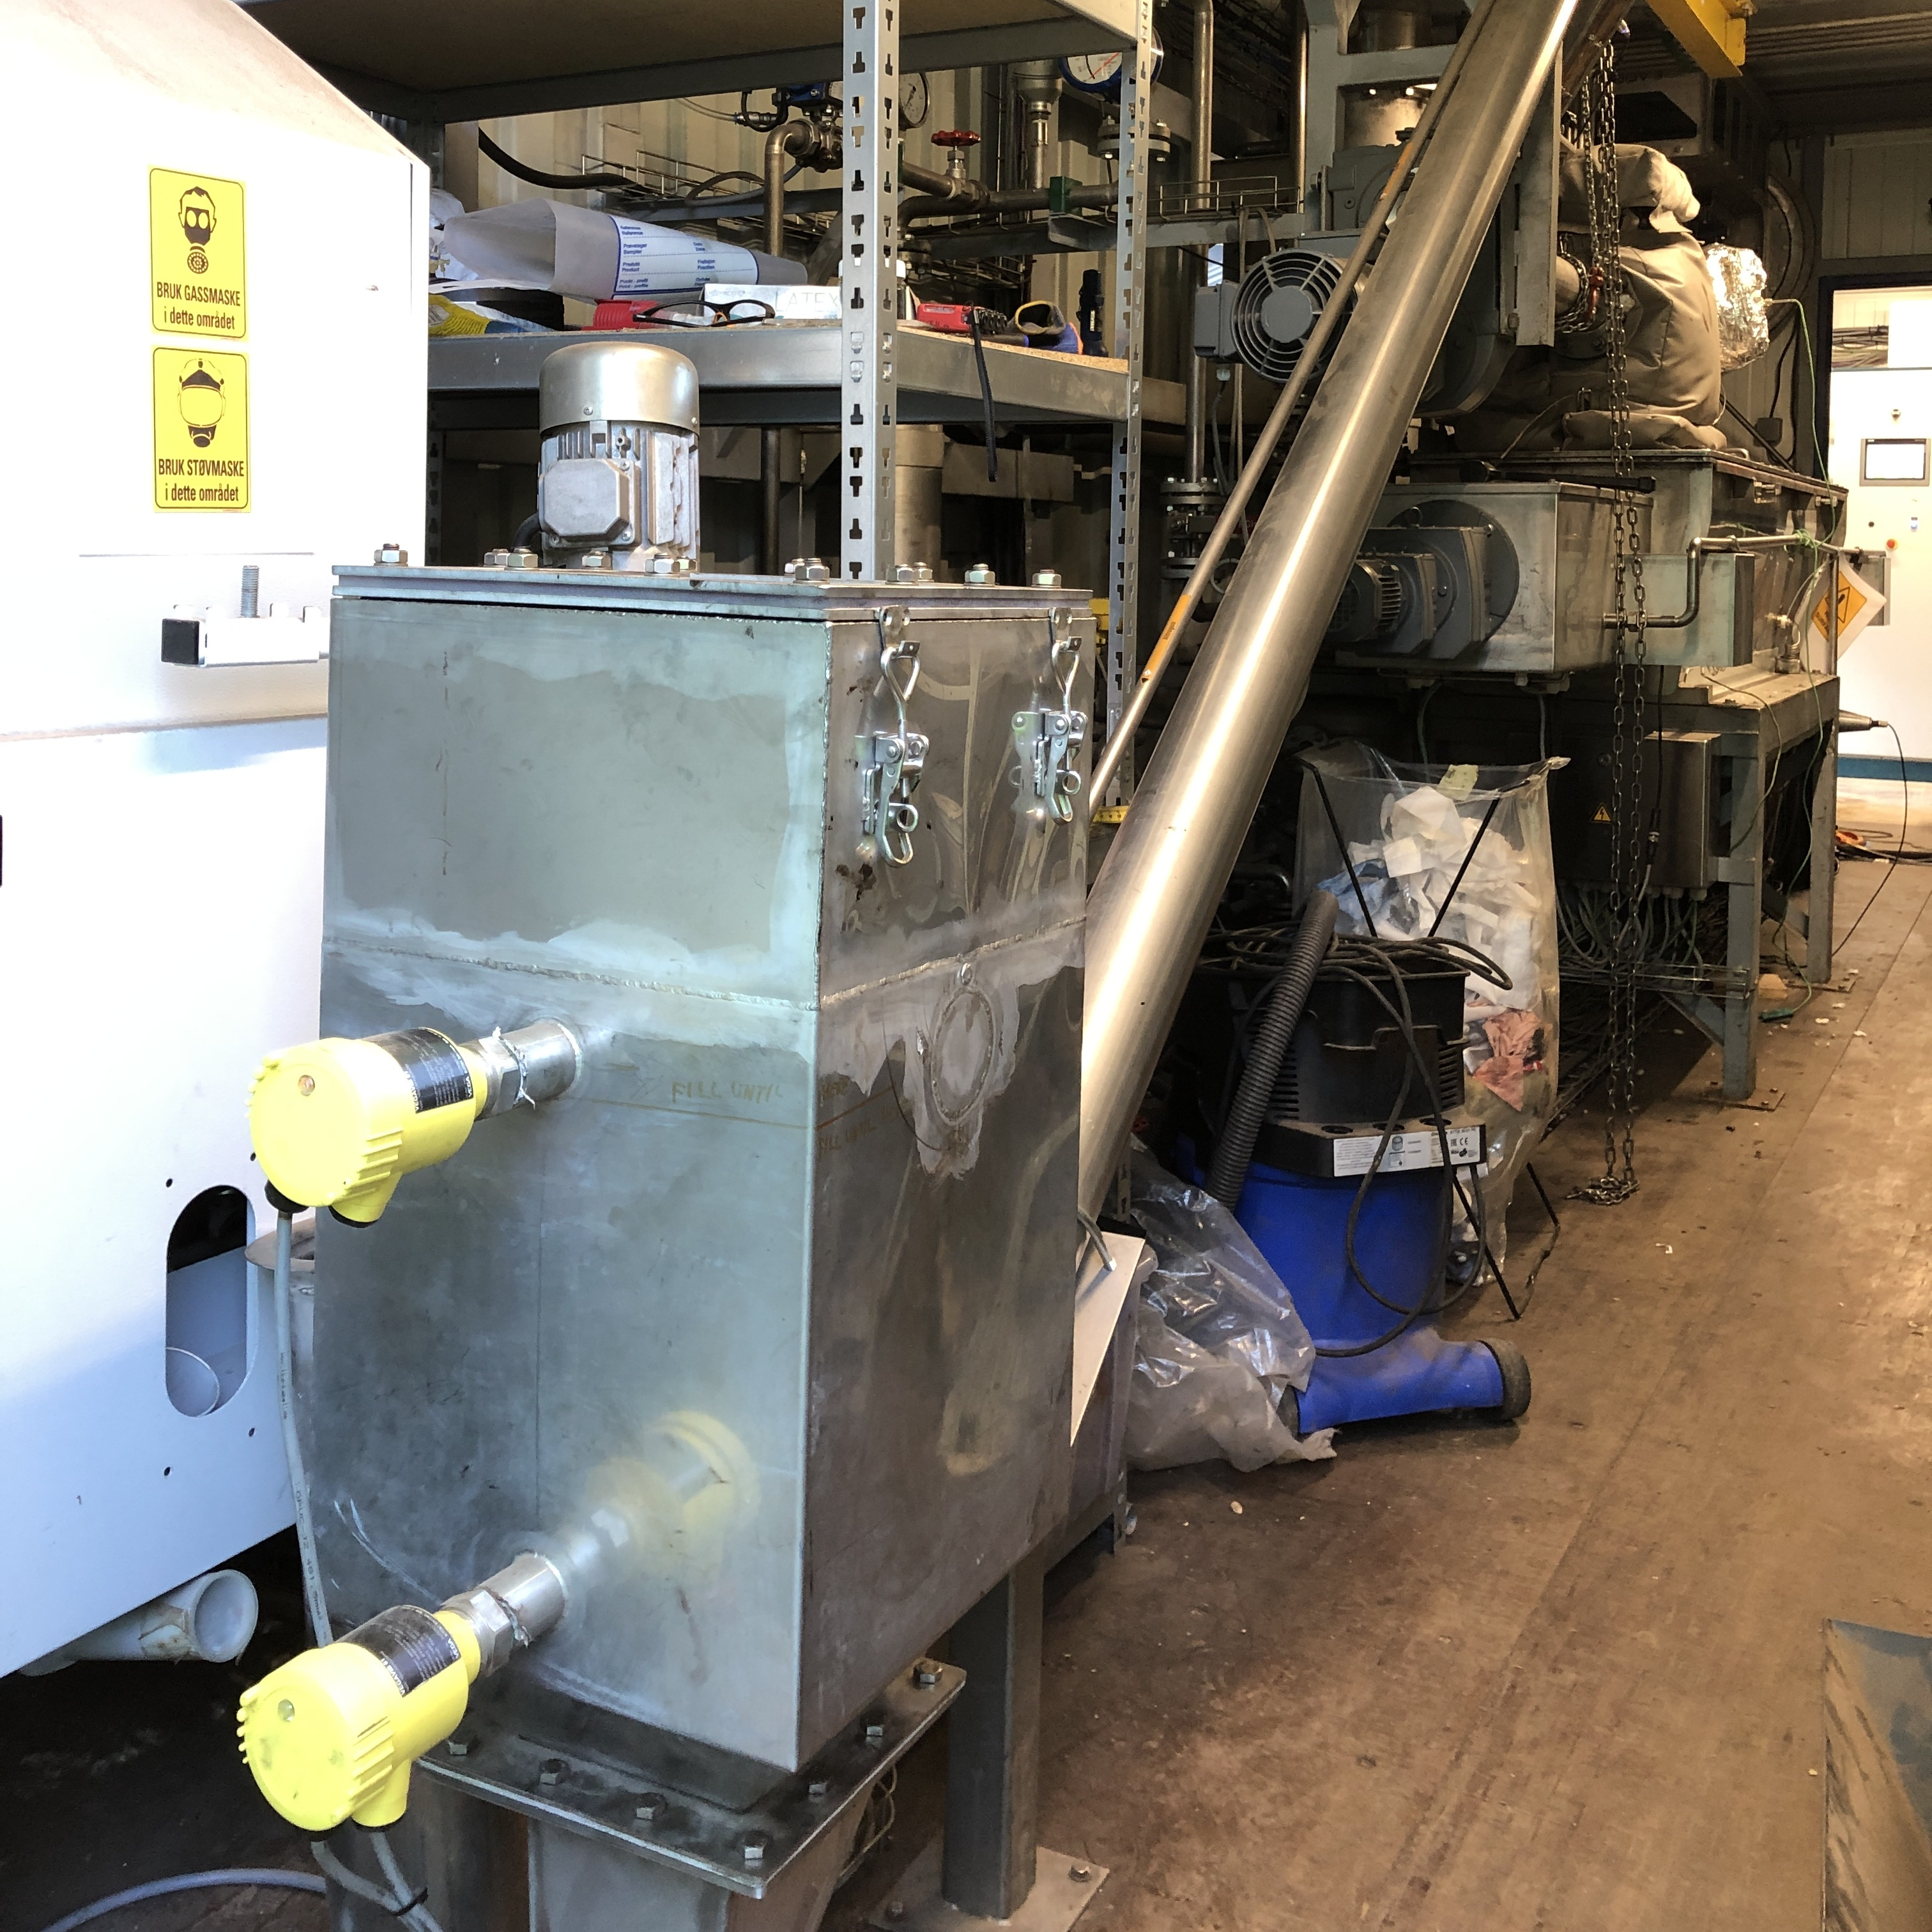
\includegraphics[width=0.6\linewidth,scale=0.6]{Bilder/Pyrolysis/Feeder.jpg}
    \caption{Starting point for the pyrolysis process where feedstock pellets are added to the system and transported with a rotating screw up the pipe on the photo that leads to the pyrolysis chamber.}
    \label{fig:feeder}
\end{figure}

\begin{figure}
    \centering
     \begin{subfigure}[t]{\linewidth}
         \centering
         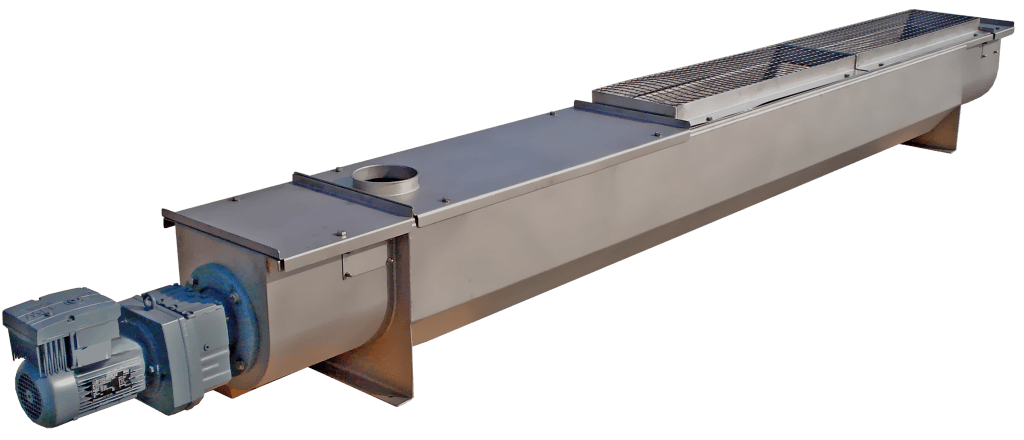
\includegraphics[width=0.74\linewidth,scale=0.74]{Bilder/Pyrolysis/PyrolyzerChamber.png}
         \caption{}
     \end{subfigure}
    \centering
    \begin{subfigure}[b]{\linewidth}
         \centering
         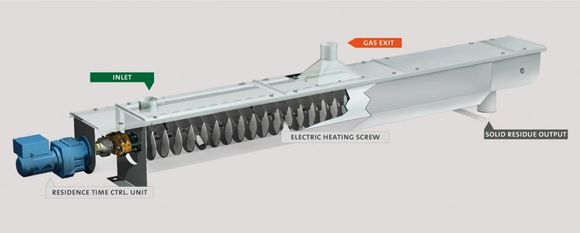
\includegraphics[width=0.74\linewidth,scale=0.74]{Bilder/Pyrolysis/spirajoule.jpeg}
         \caption{}
     \end{subfigure}
    \caption{\textbf{(a)} external view of the pyrolysis chamber, \textbf{(b)} internal view of the pyrolysis chamber. The Spirajoule\textsuperscript{\textregistered} is heated to the desired pyrolysis temperature and the speed of rotation is set to the wanted residence. Adopted from \url{https://www.biogreen-energy.com/spirajoule}.}
    \label{fig:pyrolysischamber}
\end{figure}

\begin{figure}
    \centering
    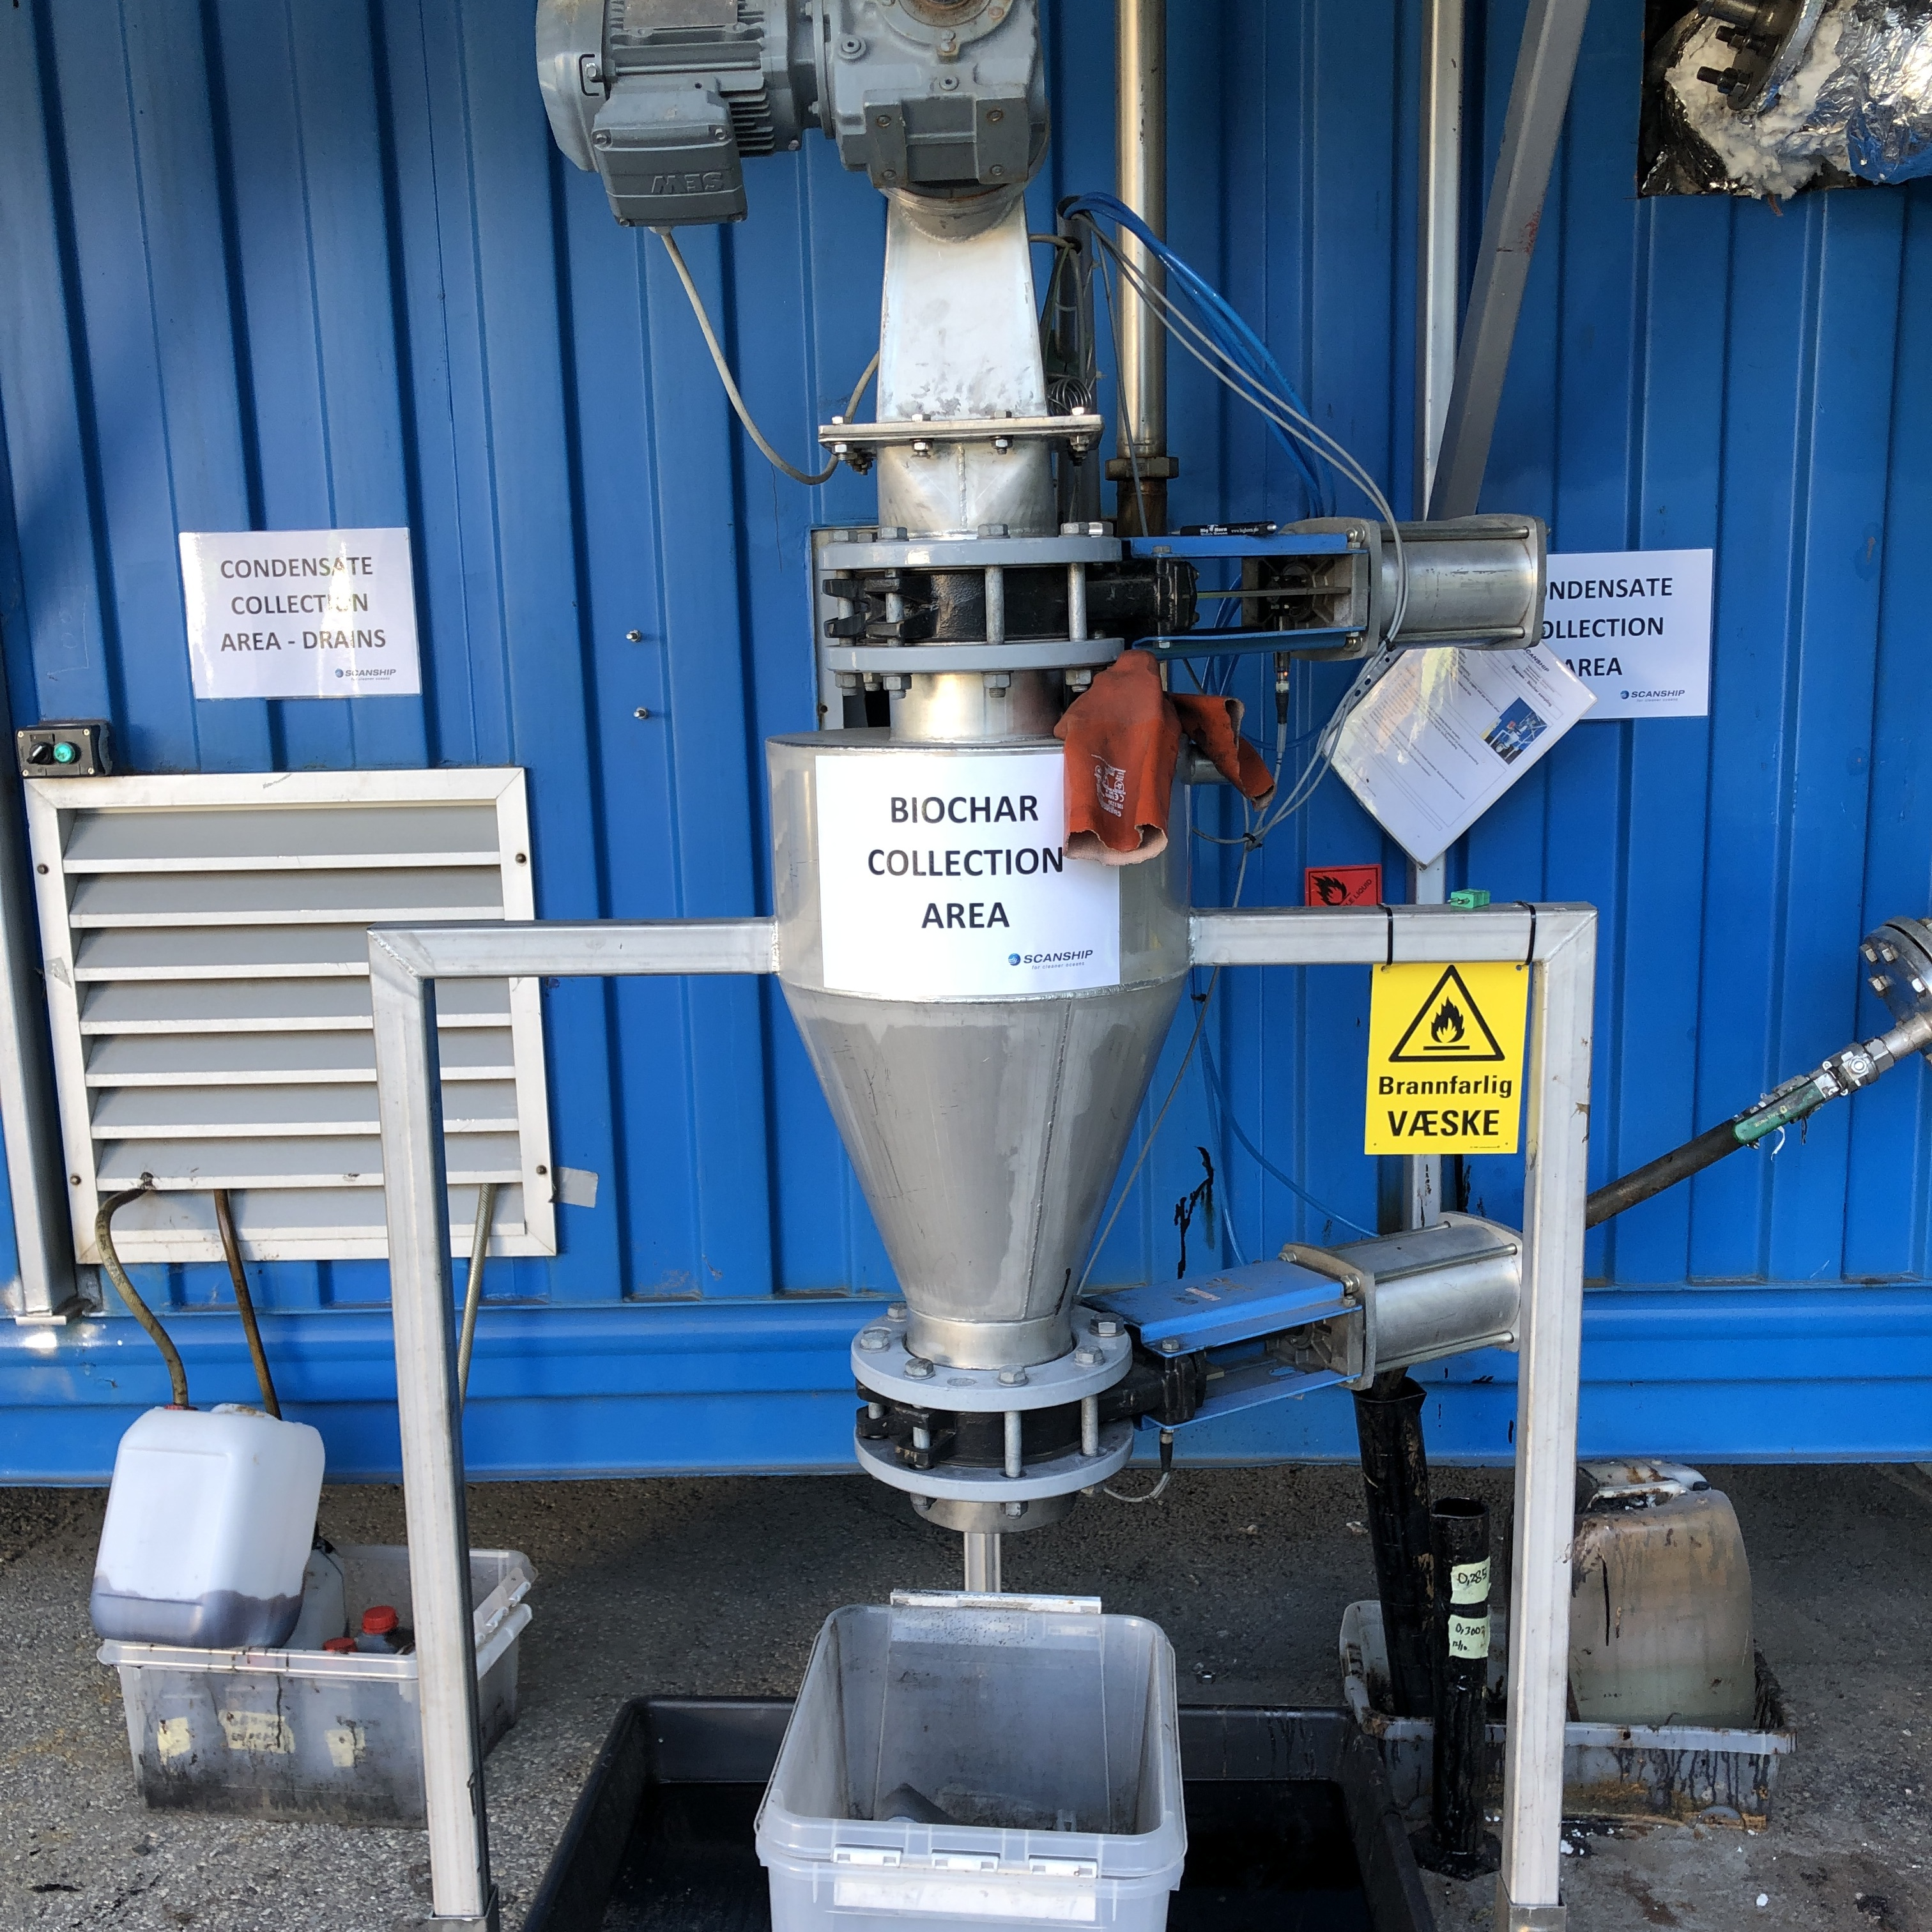
\includegraphics[width=0.6\linewidth,scale=0.6]{Bilder/Pyrolysis/BiocharCollection.jpg}
    \caption{Biochar collection area.}
    \label{fig:biocharCollection}
\end{figure}

\begin{figure}
    \centering
    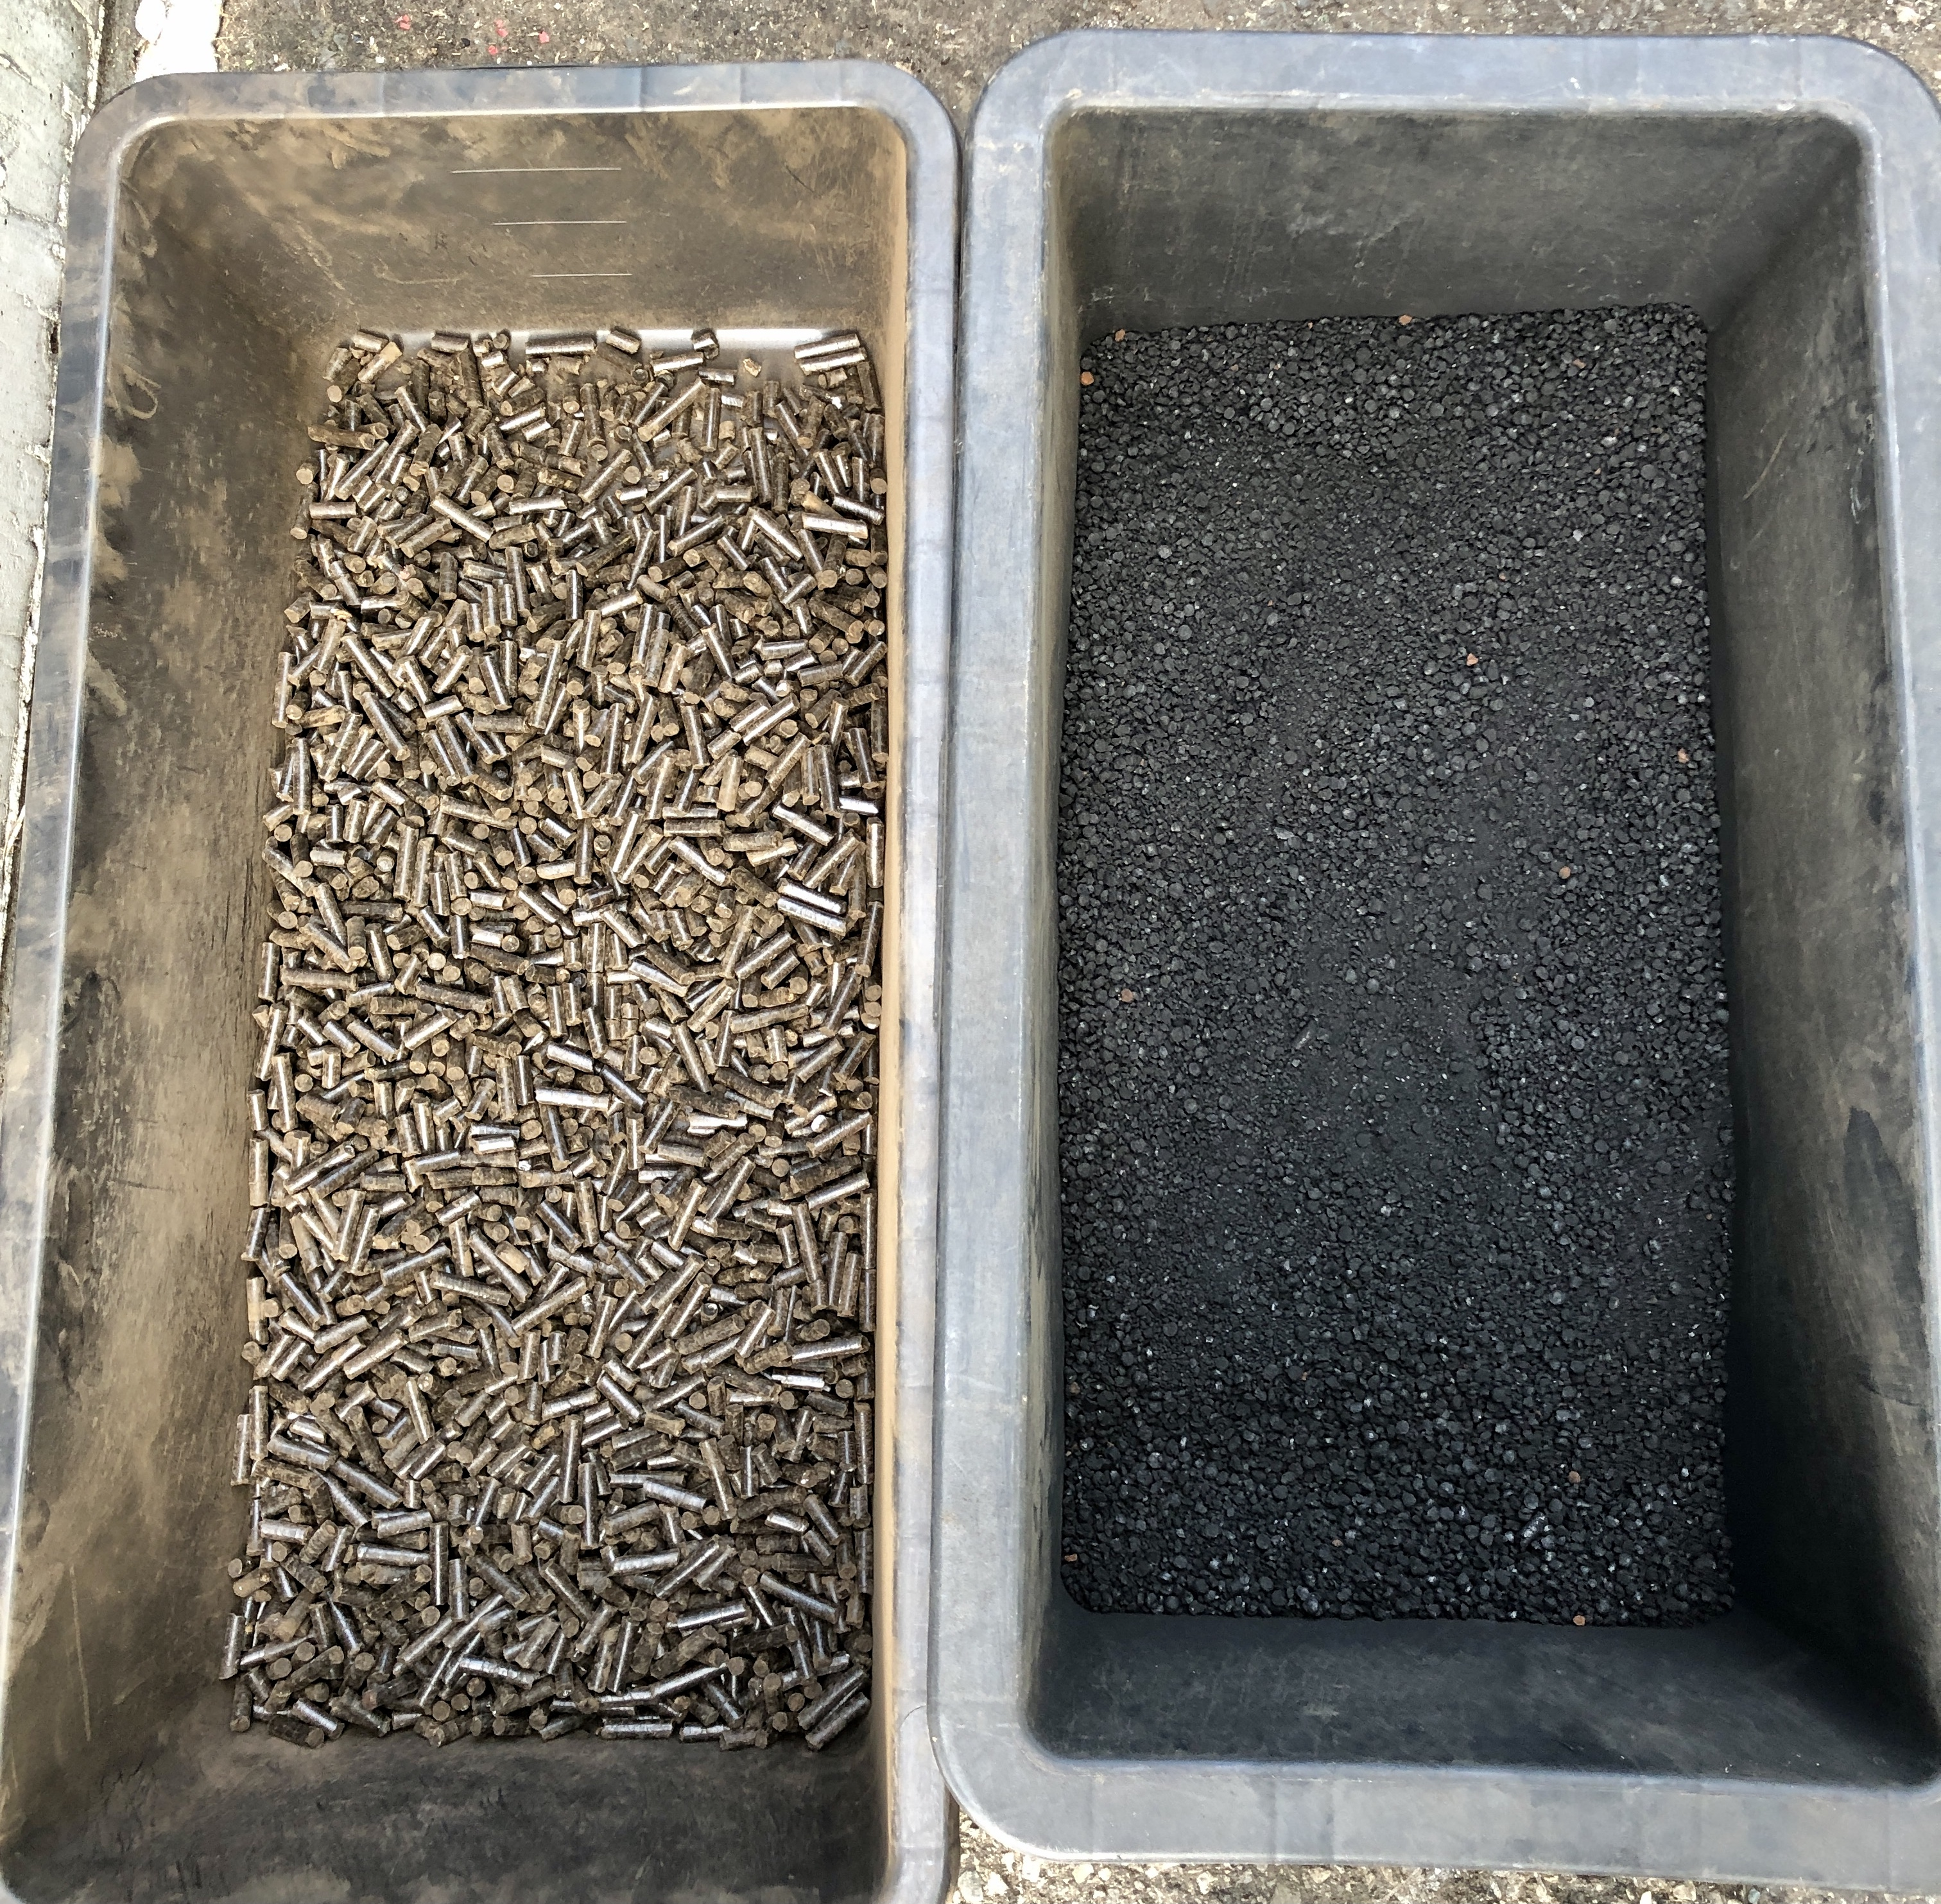
\includegraphics[width=0.6\linewidth,scale=0.6]{Bilder/Pyrolysis/Pellets.png}
    \caption{Feedstock pellets (left) and pyrolyzed pellets/biochar (right) of digested sludge Lindum (DSL).}
    \label{fig:pellets}
\end{figure}

The syn-gas from pyrolysis is led through a condensing pipe (double pipe with cold water injected in the outer pipe). Syn-gas condenses into bio-oil at two points. The first condensate consists of oils with the higher-range boiling points, i.e., long-chain hydrocarbons. The second condensate are oils with lower boiling points, i.e., lighter molecules. Syn-gas that does not condense at this point is led into a combustion chamber where a steady inflow of propane ensures a clean burning process of the remaining molecules into CO$_2$ and H$_2$O which is emitted through the chimney. See \cref{appSec:pollution} for additional work on measurements on environmental pollutant emission from the ETIA unit.

\begin{figure}
        \centering
         \begin{subfigure}[t]{\linewidth}
         \centering
         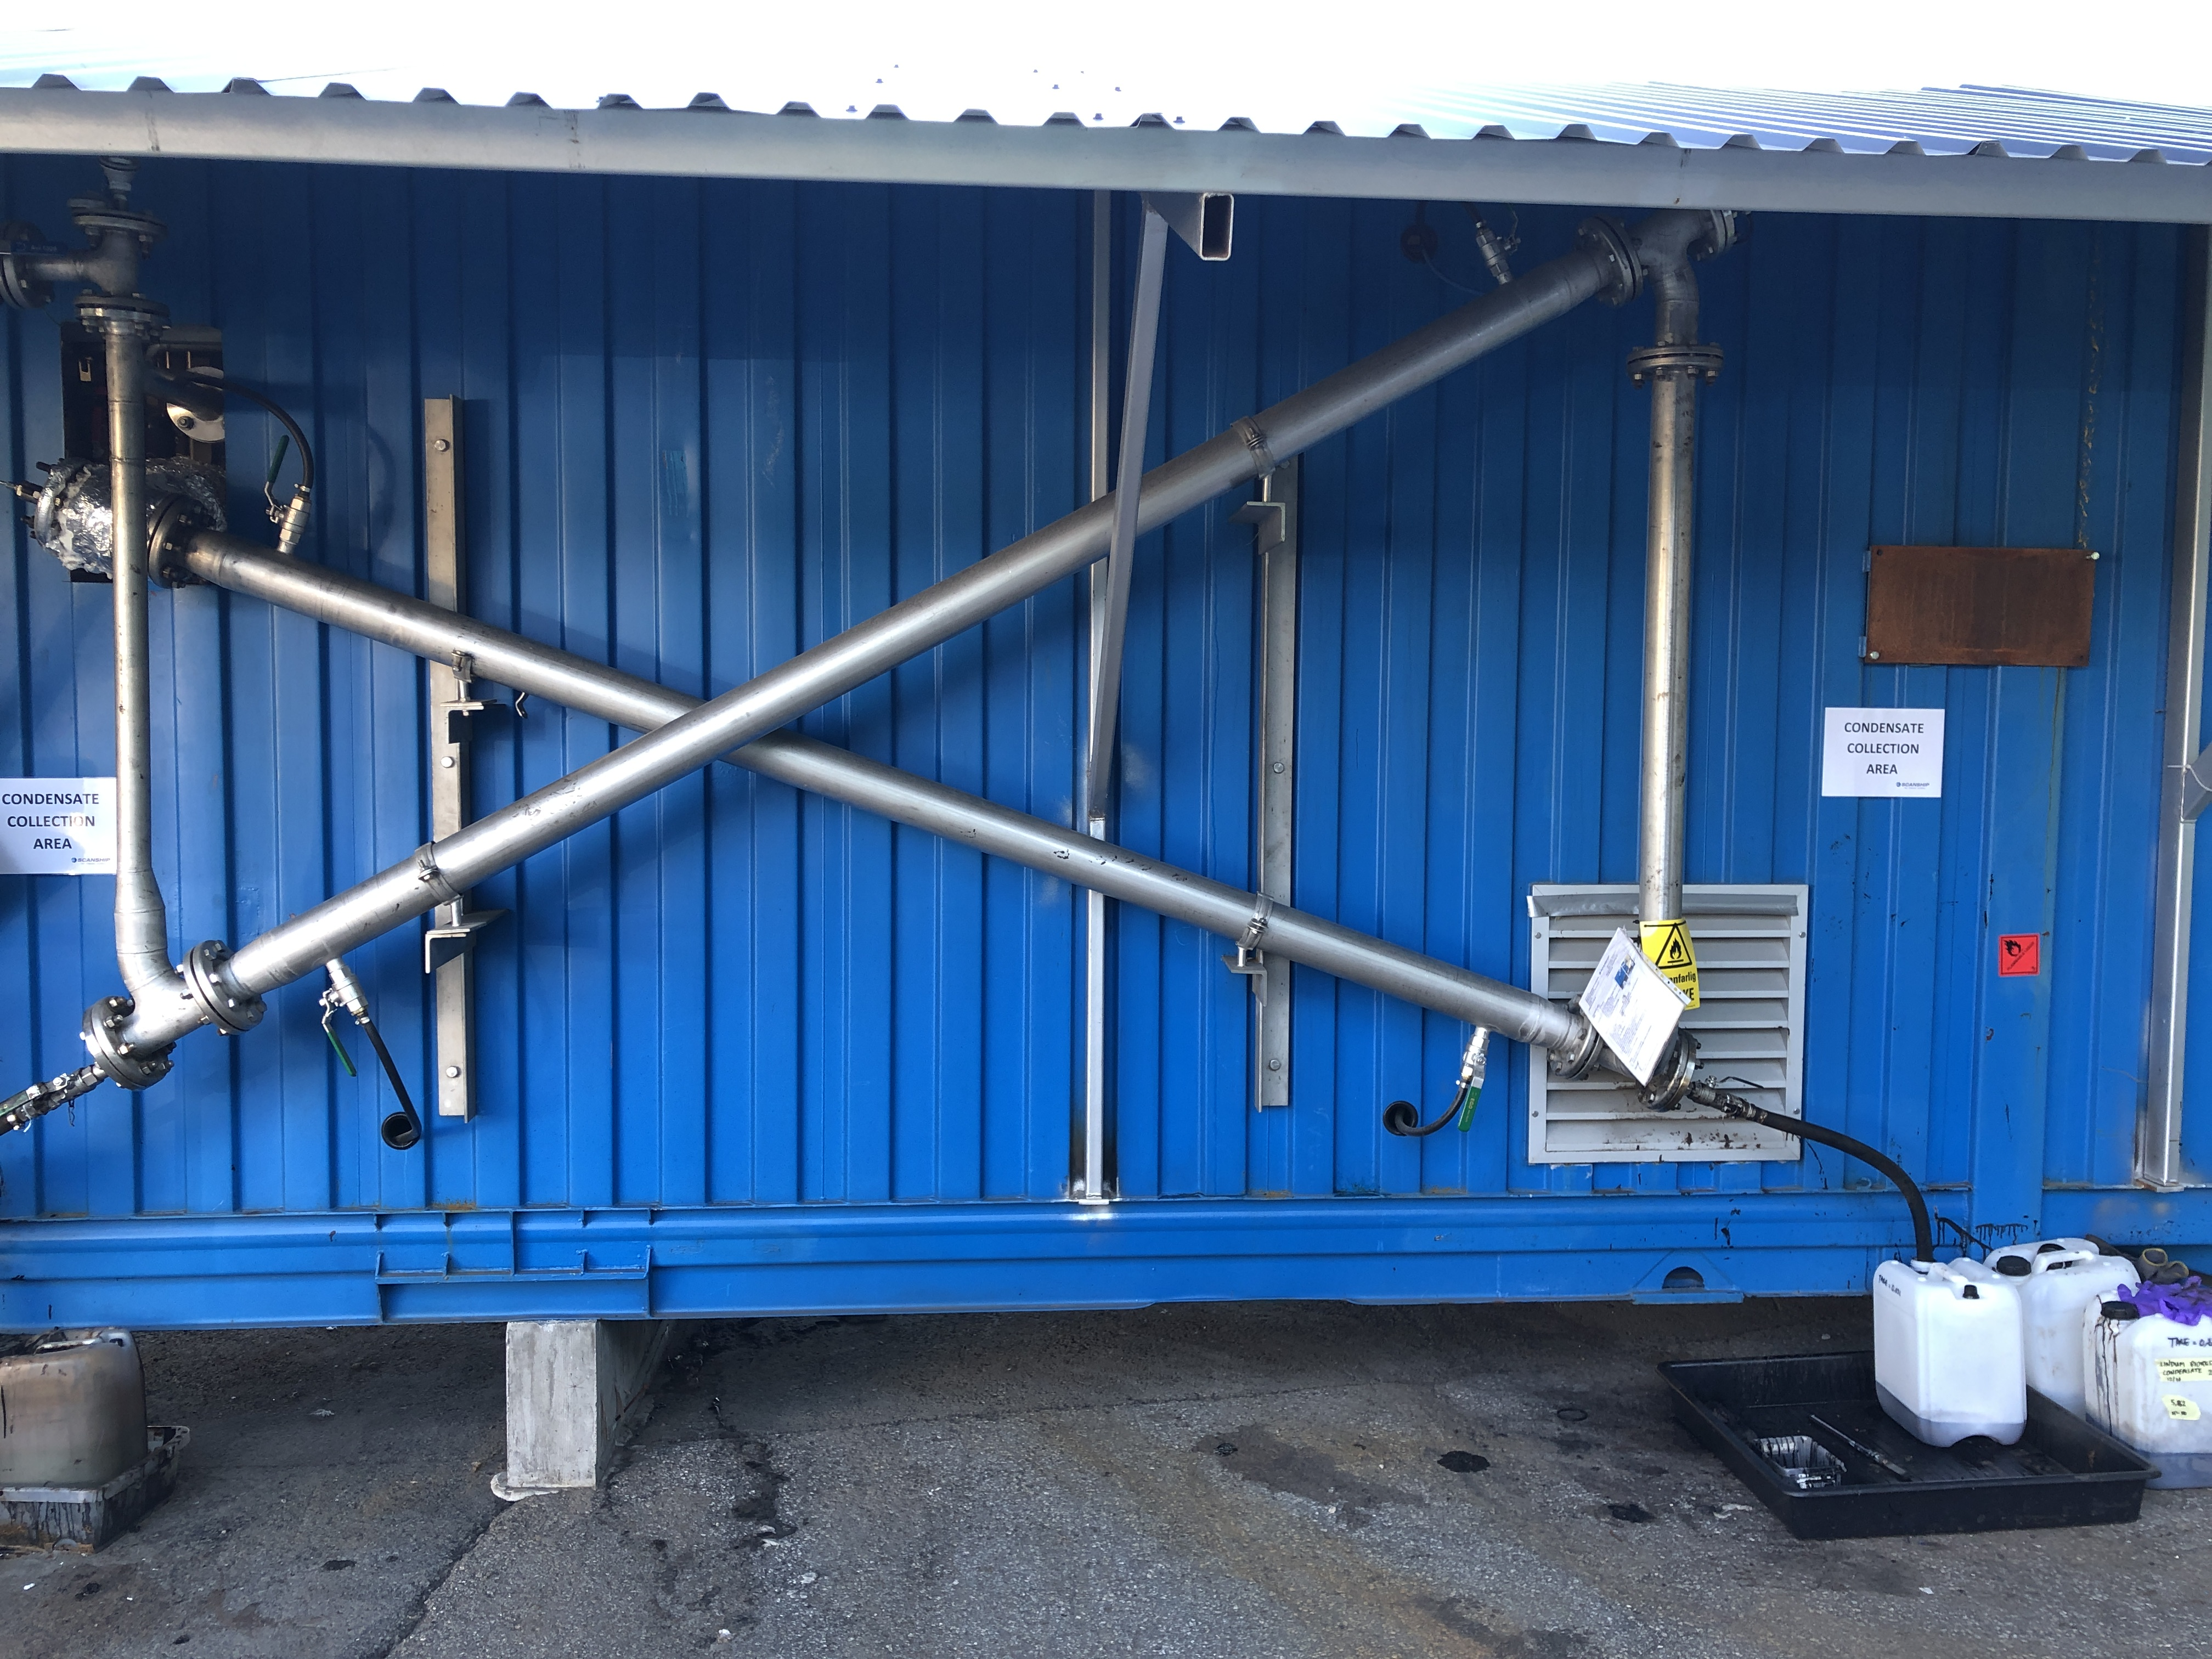
\includegraphics[width=0.74\linewidth,scale=0.74]{Bilder/Pyrolysis/Condenser.png}
         \caption{}
         \label{fig:condenserfull}
     \end{subfigure}
           \subfloat[]{%
              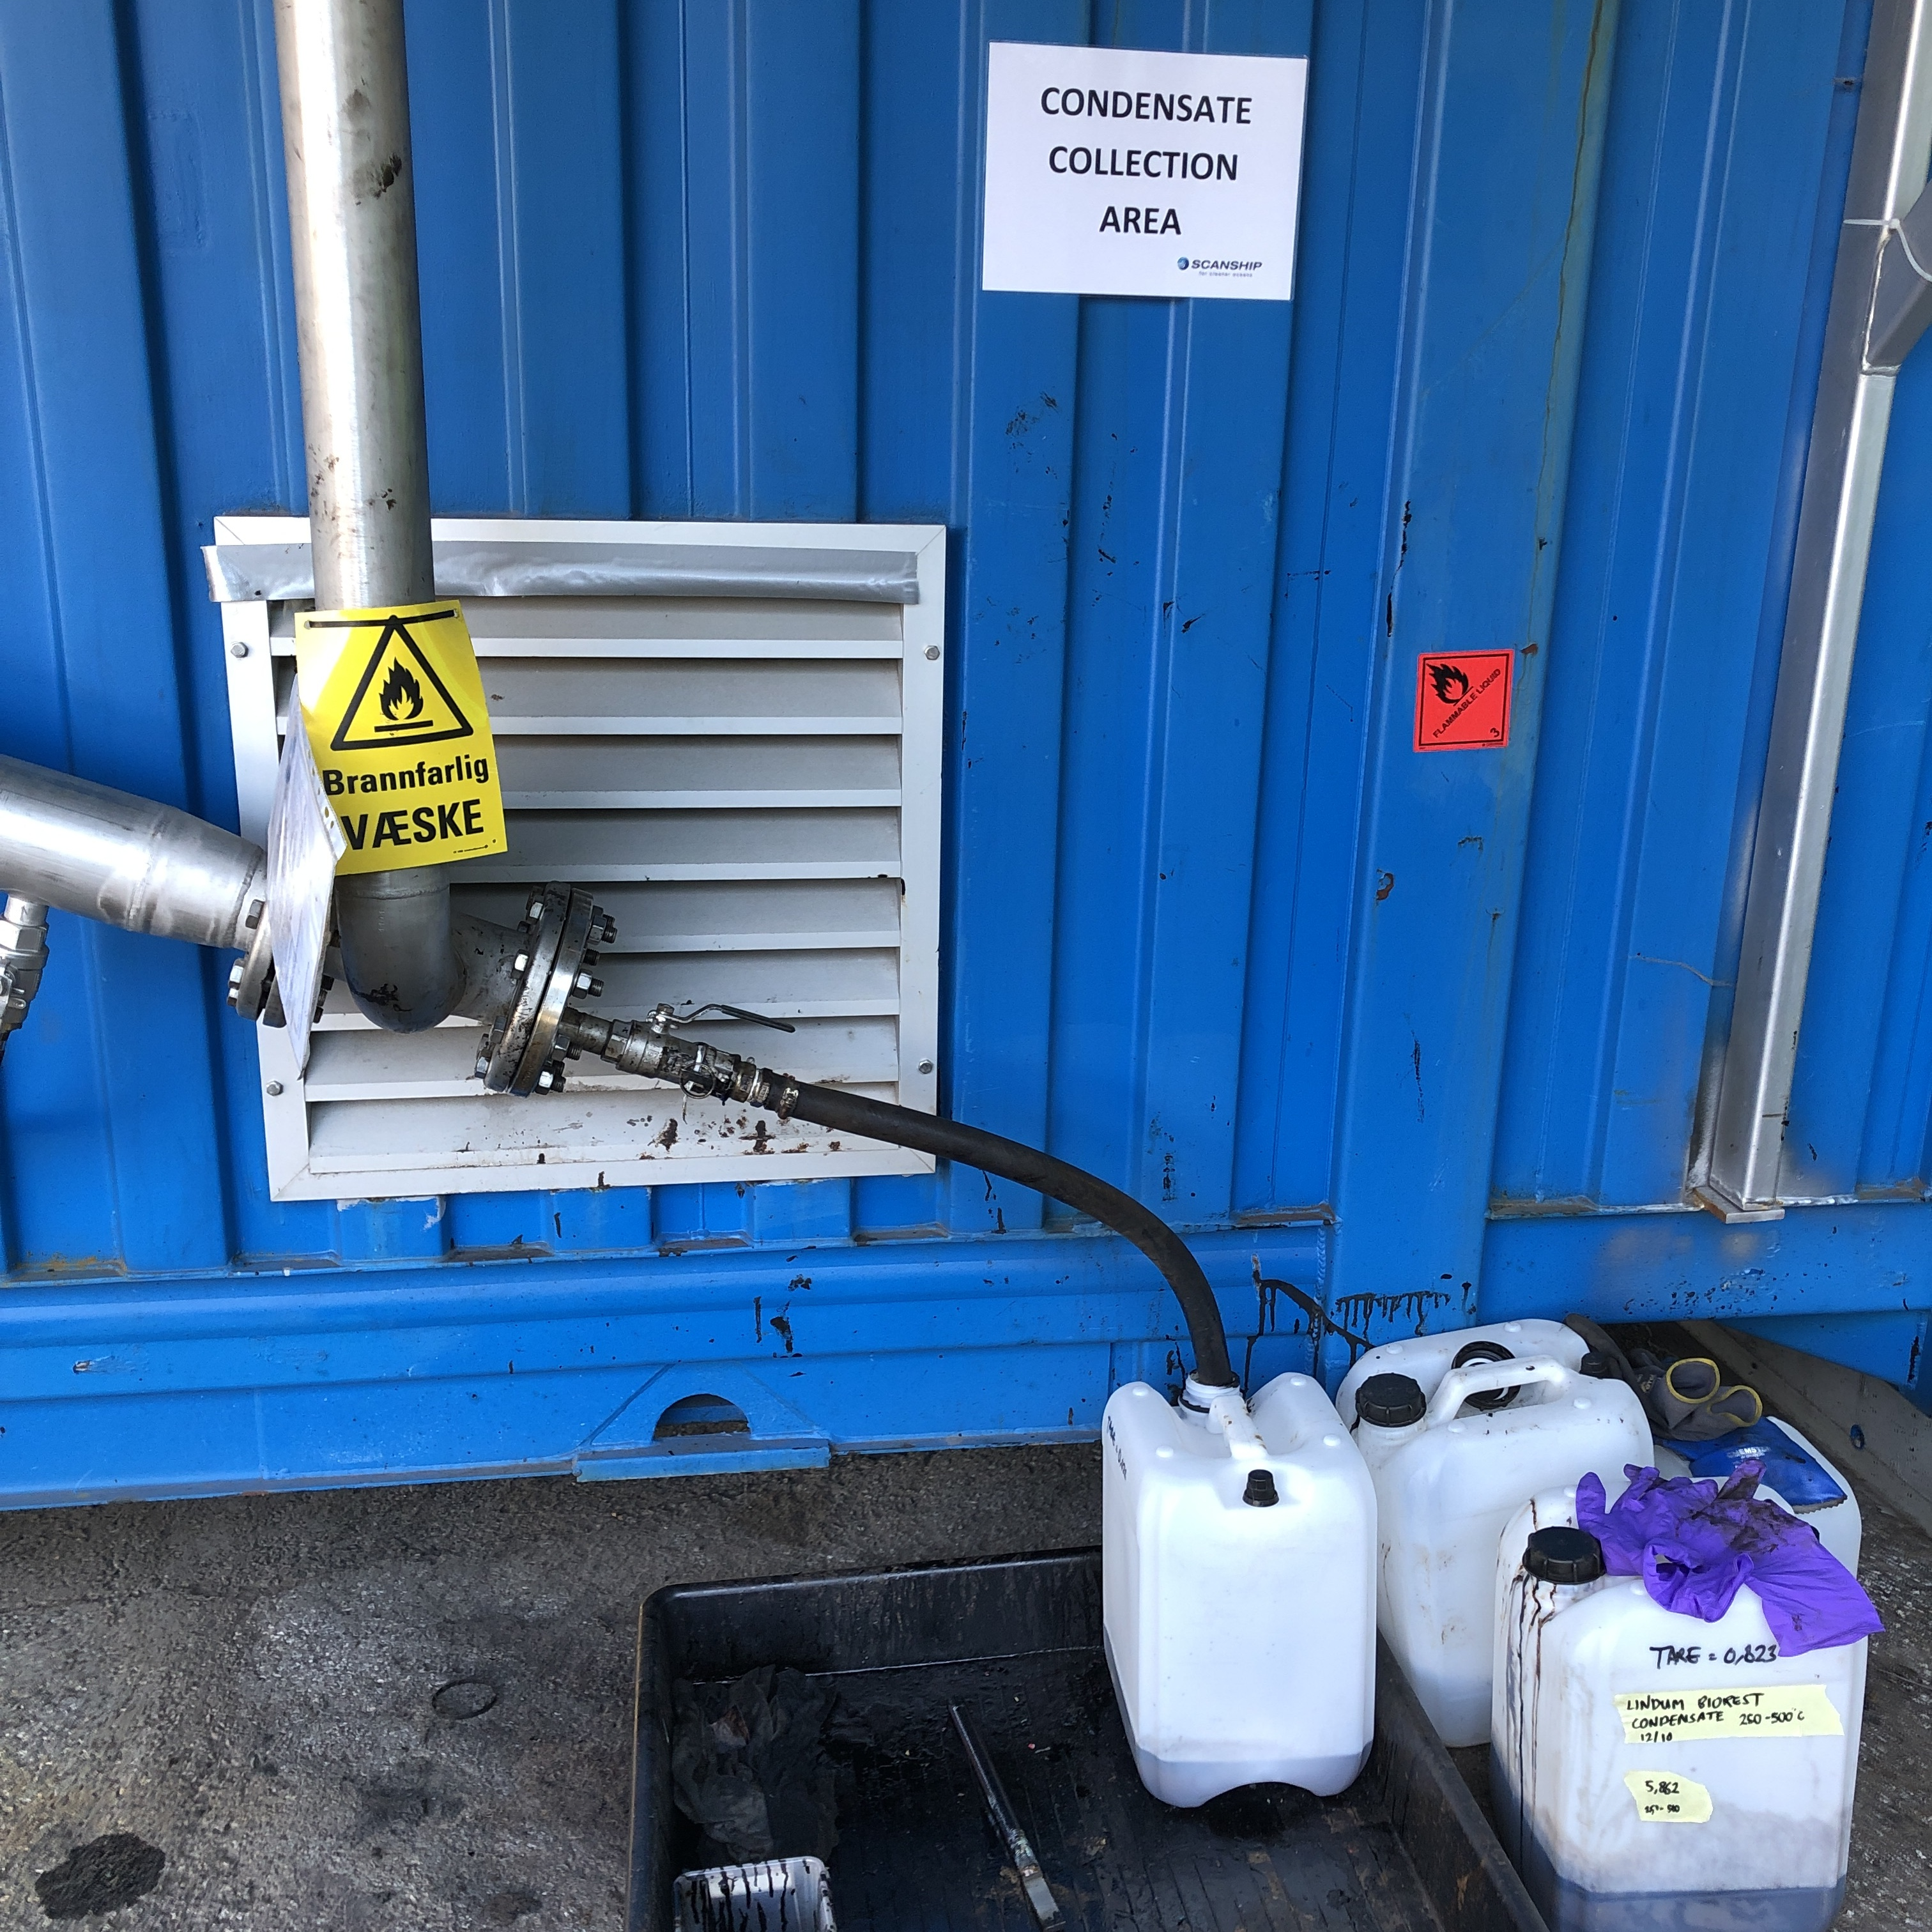
\includegraphics[height=6cm]{Bilder/Pyrolysis/CondensateCollection1.jpg}%
           }
           \hspace{0.5cm}
           \subfloat[]{%
              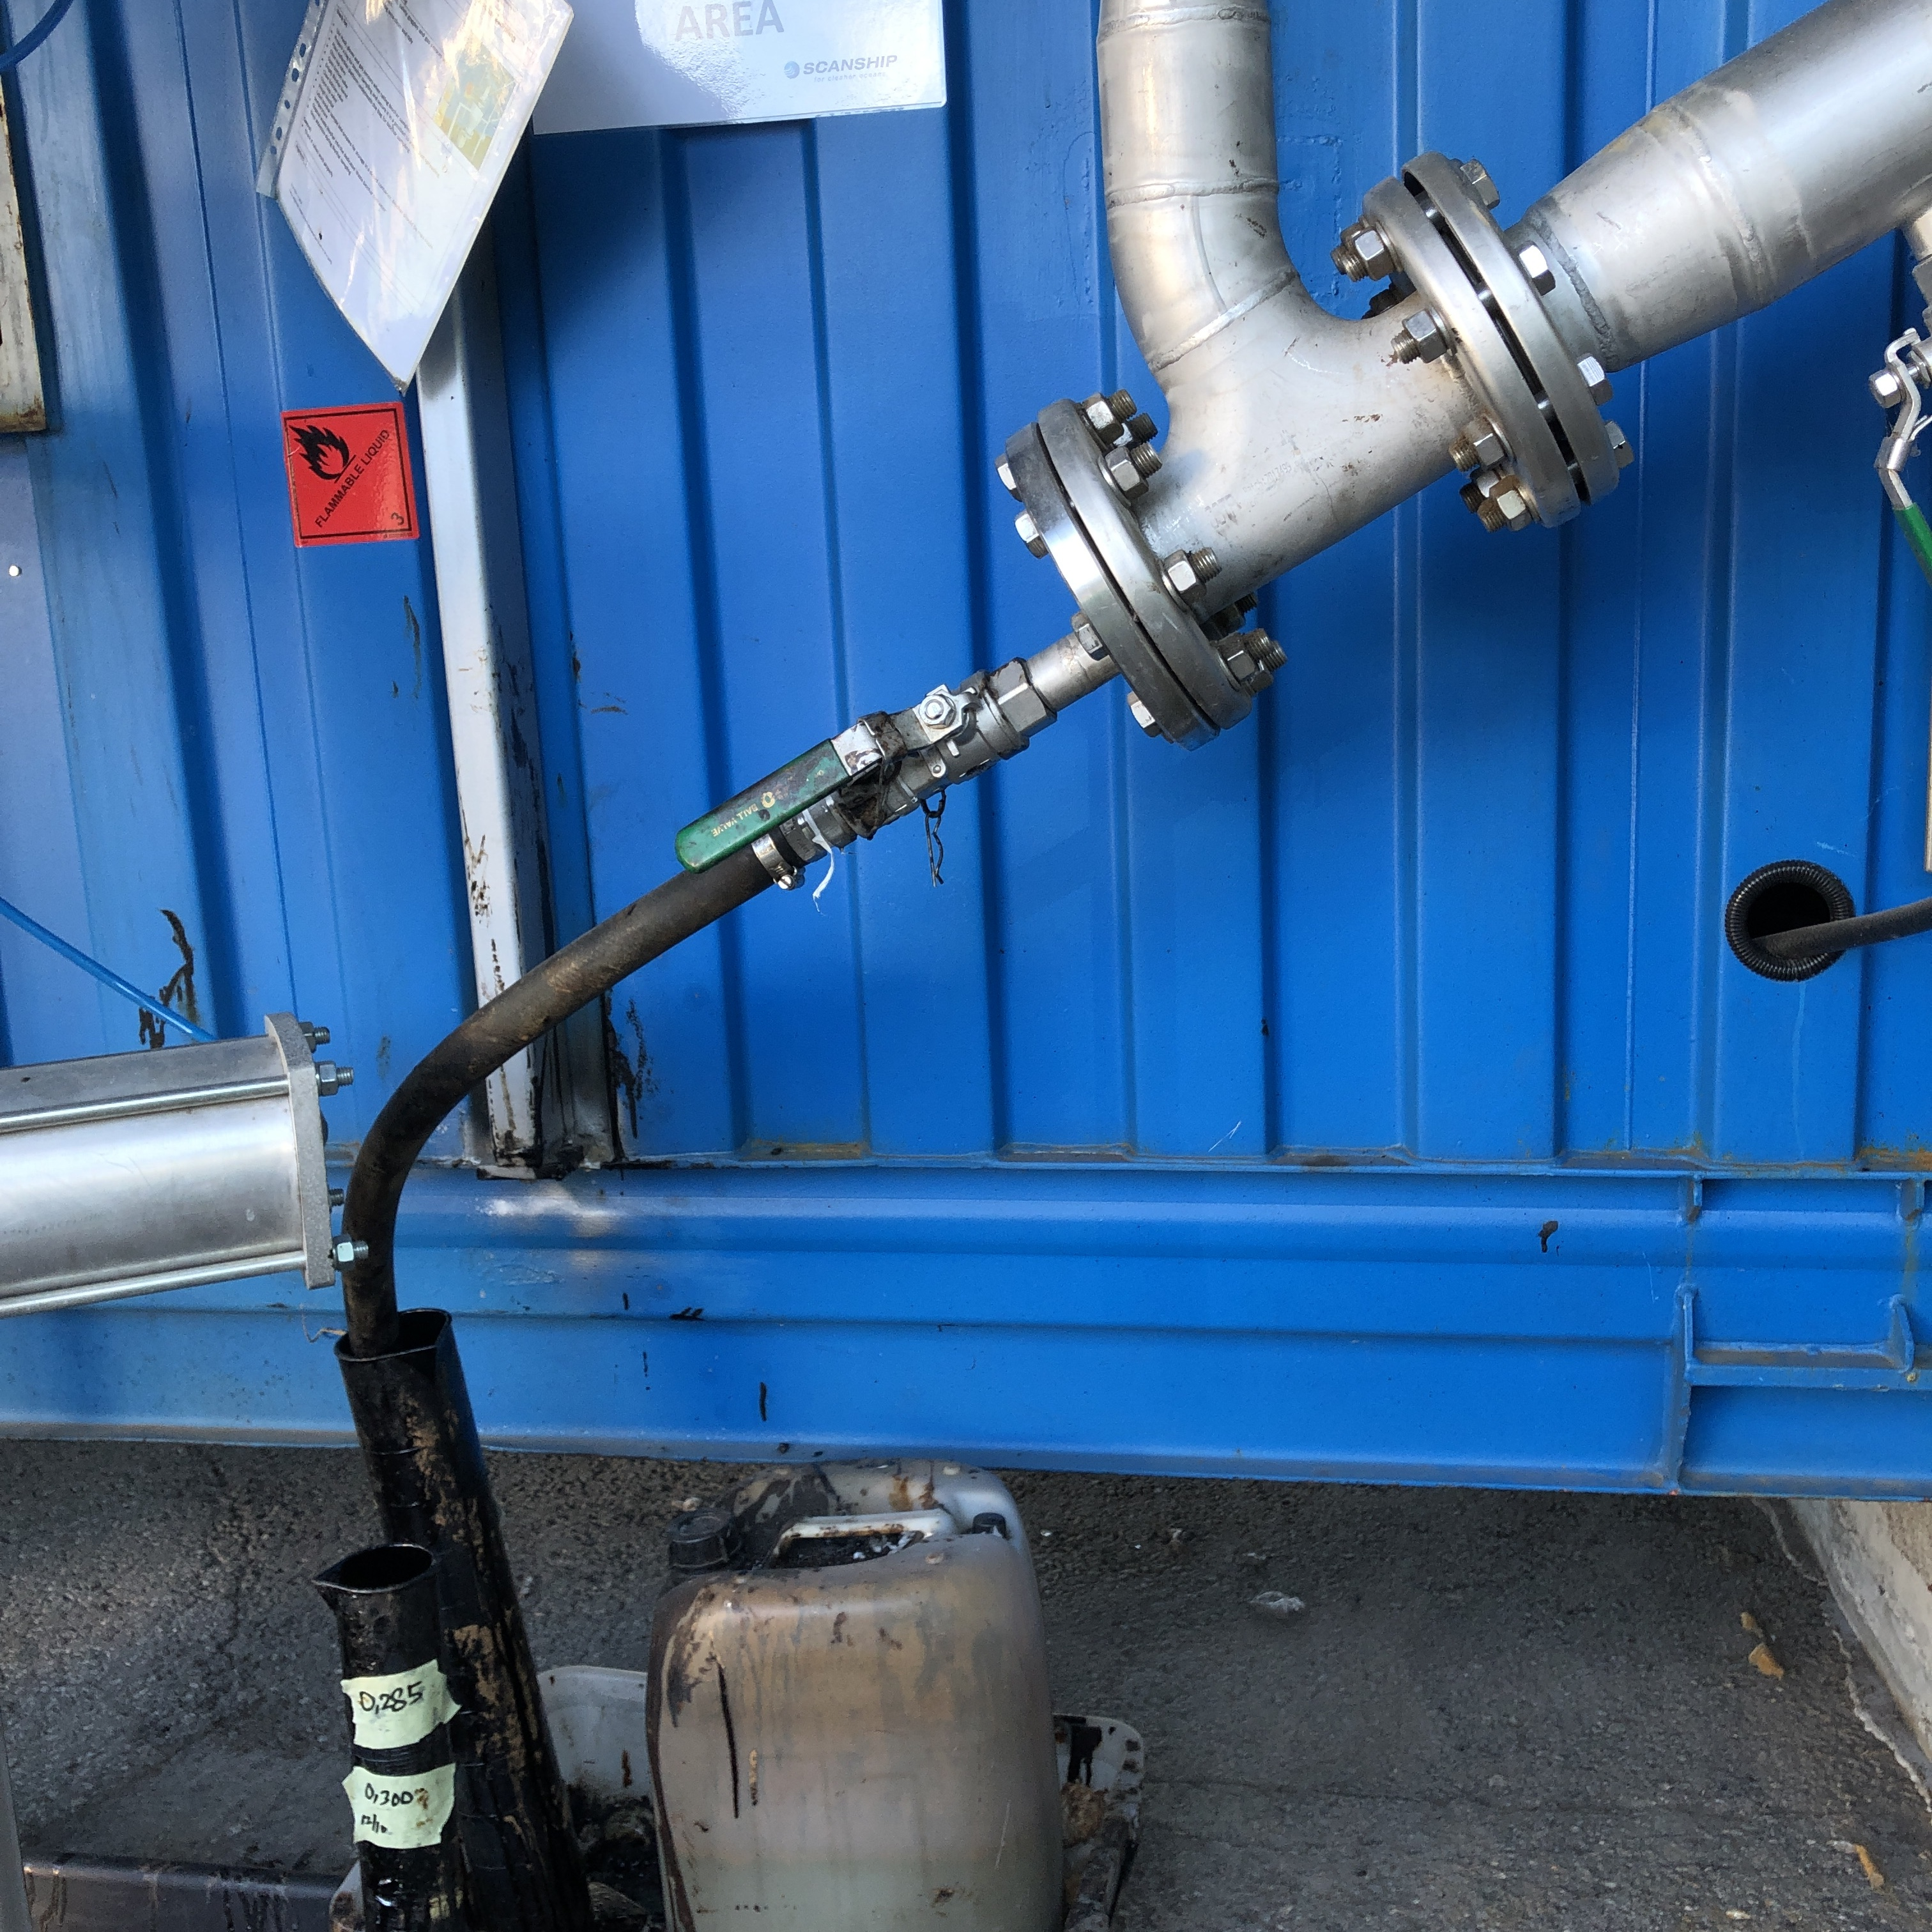
\includegraphics[height=6cm]{Bilder/Pyrolysis/CondensateCollection2.jpg}%
           }
        \caption{Syn-gas condenser. (a) First condensate collection area draining long-chain bio-oils. (b) Second condensate collection area draining short-chain bio-oils.}
        \label{fig:condenser}
\end{figure}

\subsection{Preparation of the biochar samples}
The three biochars were crushed and sieved into fine-powdered biochar (D \textless 1 mm) using a ball mill (Retsch ISO 9001) with five balls at 50 rpm for 5 minutes and transferred to LDPE zipper bags for storage (4 \textdegree C). 

%%%%%%%%%%%%%%%%%%%%%%%%%%%%%%%%%%%%%%%%%%%%%%%%%%%%%%%%%%%%%%%%%%%%%%%%%%%%%%%%%%%%%%%%%%%%%%%%%%%%%%%%%%%%%%%

\section{Biochar-water batch tests}
Sorption experiments were carried out to characterize the sorption capacity of CWC, ULS, and DSL to six perfluorinated carboxylic acids (PFCAs) of increasing chain lengths. The target analytes (TAs) were perfluoropentanoic acid (PFPeA; C5), perfluorohexanoic acid (PFHxA; C6), perfluoroheptanoic acid (PFHpA; C7), perfluorooctanoic acid (PFOA; C8), perfluorononaoic acid (PFNA; C9), and perflurodecanoic acid (PFDA; C10). All 18 sorption experiments were made as 10-point isotherms within a 10\textsuperscript{4} concentration range. 

\subsection{Design of sorption isotherms}
Determination of spike concentrations for each TA was taken as a trade-off between convenience of preparing standard solution at a certain concentration and biochar dose together with predicted biochar-water partition coefficients, K$_{BC}$ and the instrumental LOQs in LC-MS/MS. $K_{BC}$ values used for the calculations were based on a series of sorption experiments conducted on five PFCAs to activated carbon by \cite{Xiao2017}. The $K_{BC}$s used in the calculations and are listed in \cref{tab:Kbc}. The right balance between these parameters is important to ensure detectable $C_w$ across a wide enough concentration range to see a sorption trend on the isotherm. A 10$^4$ concentration range was selected. The relationship between $K_{BC}$ (L g\textsuperscript{-1}), the sorbed concentration, $C_s$ (\textmu g g\textsuperscript{-1}), and the freely dissolved aqueous concentration, $C_w$ (\textmu g L\textsuperscript{-1}) is expressed as:

\begin{align}
    \label{eq:Kbc1}
    K_{D} = \frac{C_s}{C_w}
\end{align}

\cref{eq:Kbc1} can be rearranged to calculate $C_w$ based on the mass TA spiked to each sample and the estimated $K_D$:

\begin{align}
    \label{eq:Cw2}
    C_w=\frac{\frac{m_{tot}}{\left (\frac{m_{BC}\times K_{BC}}{V_w}\right)+1}}{V_w}
\end{align}

Where $m_{TA}$ is the mass TA spiked, $m_{BC}$ is the biochar dose, and $V_w$ is the volume of the sample matrix.The lowest spike concentration for each isotherm was calculated as the $C_w$ to be two times the method LOQ for the LC-MS/MS instrument in at NTNU, Trondheim using \cref{eq:Cw2}.

\begin{table}
\centering
\caption{Biochar-water distribution coefficients ($K_{BC}$) for PFCAs based on \cite{XiaoSI2017}.} \label{tab:Kbc}
\begin{threeparttable}
    \begin{tabular}{@{}lcc@{}}
    \toprule
    \multicolumn{1}{l}{\begin{tabular}[l]{@{}l@{}}Compound\end{tabular}} &  \multicolumn{1}{c}{\begin{tabular}[c]{@{}c@{}}log $\mathrm{K_{BC}}$\\ \citep{XiaoSI2017}\end{tabular}} & \multicolumn{1}{c}{\begin{tabular}[c]{@{}c@{}}est. log $\mathrm{K_{BC}}$ \end{tabular}} \\ \midrule
    PFPeA & 4.16 & 4.16 \\
    PFHxA & 4.15 & 4.15 \\
    PFHpA & 4.49 & 4.49 \\
    PFOA & 4.76 & 4.76 \\
    PFNA & *4.89 & 4.89 \\
    PFDA & *5.09 & 5.09 \\ \bottomrule             
    \end{tabular}
\begin{tablenotes}
\item * not included in \citep{XiaoSI2017}, so the values are extrapolated from the shorter chain lengths.
\end{tablenotes}
\end{threeparttable}
\end{table}

A preliminary sorption test was conducted to compare the $K_{BC}$ values selected from the literature to ULS and CWC. DSL was not included in the screening because it was not yet produced. The batch tests were performed using a mid-range concentration of PFOA (1335 {\textmu}g/L) and 1 g CWC and 100 mg ULS in 50 mL PP tubes. The aqueous concentration in the two test tubes were determined according to DIN38407-42 by the accredited laboratory Eurofins Norway. Sorption of PFCA to ULS was expected to be lower than for CWC. However, the test run for sorption of PFOA to ULS showed sorption two orders of magnitude higher than expected. Therefore, the same $K_d$ values were used for calculating spike concentrations for the three biochars. A 100 mg biochar dose was decided to be ideal to balance convenient spike concentrations with sufficient sorption. In summary, the same analyte spike concentrations and biochar doses were used to make the isotherms for CWC, ULS and DSL.

\subsection{Preparation of PFCA analytical standards}\label{ssec:PFCAanalytic}
Methanol stock solutions were prepared for the six target PFCAs. The liquid/crystalline PFCAs were weighed on an analytical scale and transferred to 10 mL volumetric flasks. Anhydrous methanol (99.8\%) was used as solvent for the first stock solutions to assure complete dissolution. Two working standards for each PFCA were prepared from the PFCA-MeOH stock solutions in volumetric flasks (STD11 and STD12 \cref{appTab:expConc}) and were stored at room temperature and light conditions during the experimental period. 

The concentration of the working standards were corrected for by quantification with LC-MS/MS of a 2-time diluted standard at an optimum concentration for the instrument calibration curve (10-20 \textmu g L\textsuperscript{-1}, \cref{appSec:IsothermSetup}, \cref{appTab:expConc}).

%UPDATE WITH CORRECTED VALUES!!!!!!!
\begin{table}
    \caption{Spike concentrations for each PFCA batch test.}
    \label{tab:concentrations}
    \adjustbox{max width=\textwidth}{%
    \begin{tabular}{lrrrrrrrrrr}
    \toprule
    & \multicolumn{10}{c}{{[}PFAS{]}   (\textmu g/L) spiked} \\ \midrule
    Compound & SP1 & SP2 & SP3 & SP4 & SP5 & SP6 & SP7 & SP8 & SP9 & SP10  \\ \midrule
    PFPeA & 0.03 & 33 & 68 & 100 & 135 & 168 & 200 & 235 & 268 & 300 \\
    PFHxA & 0.06 & 68 & 133 & 200 & 265 & 335 & 400 & 465 & 530 & 600 \\
    PFHpA & 0.01 & 13 & 28 & 43 & 57 & 73 & 88 & 103 & 118 & 130 \\
    PFOA & 0.12 & 132 & 267 & 400 & 535 & 668 & 800 & 935 & 1 070 & 1 200 \\
    PFNA & 0.16 & 178 & 355 & 535 & 711 & 890 & 1 070 & 1 245 & 1 425 & 1 600 \\
    PFDA & 0.50 & 555 & 1 110 & 1 665 & 2 220 & 2 775 & 3 330 & 3 885 & 4 440 & 5 000 \\ \bottomrule
    \end{tabular}}
\end{table}

\subsection{Preparation of biochar-water batch samples}
The same ten concentrations were used to spike the CWC, ULS and DSL batch tests. 100 mg $\pm$ 4 mg (n=60) CWC was weighed on an analytical scale and placed into pre-rinsed (50\% methanol) 50 mL PP tubes. The tubes were filled half up of Milli-Q water. In each tube, stock PFCA was pipetted using micro- (5-50 {\textmu}l and 200-1000 {\textmu}L) and milli pipettes (2-10 mL) into the char-water solution to make 10 dilutions for each of the 6 PFCAs in even intervals within the concentration points in \cref{tab:concentrations}. The tubes were filled with Milli-Q water to 50 mL. The tubes were then refilled with water to 50 mL using a glass pipette. The tubes were capped and inverted three times to remove any air bubbles. This was repeated for ULS. 

For DSL the same concentrations of PFCAs were spiked, but 50 mL was weighed on an analytical scale instead of by eye measurement to increase precision and accuracy (\cref{appSec:IsothermSetup}, \cref{appTab:milliQ}).

The char-water suspensions were assured to contain \textless 10\% MeOH. The sorbent-sorbate mixtures were shaken end-over-end (9 rpm) and/or agitated on a shaking table (160 rpm) in room temperature (20\textdegree C) for at least 14 days to reach equilibrium (based on what?). Why is it important to reach equilibrium in this study? Not kinetics we are looking at. 

\subsubsection{Cocktail batch test}
A cocktail batch test was prepared for the three biochars at SP10 to compare with C$_w$ at SP10 for the single compound batch test to determine a competition factor between the other PFCAs in the cocktail to sorption sites on the biochar. The same dose biochar was used as for the other sorption isotherms. The cumulative CMC (critical micelle concentration) for the six PFCAs at SP10 was assured not to be an issue \citep{bhhatarai2011}. 

\section{Soil-biochar-water batch tests}
14-day sorption experiments were carried out to characterize sorption by CWC, ULS, and DSL to the selected PFCAs in the presence of soil. The batch tests were prepared as 6-point isotherms within a 10\textsuperscript{4} concentration range. 

\subsection{Soil characterization}
Soil obtained from a remote field area 17 km from Uppsala, Sweden was used for batch tests with soil, biochar and water. The soil was characterized for total element concentrations, exchangeable ions, TOC and pH by the methods... Contamination of groundwater case...

\subsection{Filtration}
The samples were filtered through a 0.45 \textmu m Minisart\textsuperscript{\textregistered} regenerated cellulose syringe filter into a PP tube. Filtering of the ULS samples saw close to complete transfer of the char to the filter paper whereas for CWC much of the char was stuck at the bottom of the syringe during filtration. A mass balance test was performed to quantify the loss of CWC (see \cref{appSec:misclab}, \cref{appTab:CWCloss}).

\subsubsection{Quality control and quality assurance}
To prevent underestimation of $C_w$, filter blanks were prepared for each PFCA in triplicates at an optimum concentration range for the instrument (see \cref{ssec:PFCAanalytic}) to correct for PFCA loss to the filter paper. 
\section{Soil PFAS extraction}
To check if the soil used in the batch tests were polluted with PFAS, the soil was extracted with MeOH and analyzed with LC-MS/MS. 

Instead of preparing a soil blank batch test,
\section{Analysis of standards}
Dilutions of the PFAS standards used to spike the batch samples were analyzed both by taking them through the SPE protocol and directly by spiking the solvent (50:50 MeOH:MQ water) directly into an LC vial for analysis with LC-MS/MS 

\section{pH and conductivity}
pH and conductivity was measured by making batch tests in triplicates for BC-water, BC-soil-water and soil-water with the same w/v ratios used in the sorption experiments (1:500 for BC-water and 1:10:500 for soil-water and BC-soil-water). The samples were stirred with a magnetic stirrer for 15 minutes and left to settle for 5 days before measurement with a pH- and conductivity meter. This to assure an equilibrium state and an equivalent of soil pore water conditions.

%%%%%%%%%%%%%%%%%%%%%%%%%%%%%%%%%%%%%%%%%%%%%%%%%%%%%%%%%%%%%%%%%%%%%%%%%%%%%%%%%%%%%%%%%%%%%%%%%%%%%%%%%%%%%%%%%%%%%%%%%%%%

\section{Instrumental analysis}
Liquid chromatography--tandem mass spectrometry (LC-MS/MS) was used for quantifying PFAS in the water samples. Reversed phase solid phase extraction (SPE) was used as sample preparation method. The analyses were conducted at the Institute of Chemistry at NTNU (Trondheim, Norway).

\subsection{SPE}
SPE is a sample preparation method used to concentrate a large-volume sample to an extract that can be submitted for analyte quantification by LC-MS/MS. The sample is passed through a cartridge with a porous sorbent polymer that strongly retains polar compounds (\textpi-\textpi bonding, hydrogen bonding and hydrophobic interaction). The sorbed analytes are then eluted with an appropriate solvent, evaporated, and finally reconstituted to the desired extract volume. All samples are spiked with a mix of internal standards (ISs) to compensate for variations in extraction percentages and instrumental response by the MS/MS detector \citep{arvaniti2014}. To minimize risk of contamination during laboratory work, working benches were cleaned with acetone and covered with aluminum foil. Sterilized PP tubes were used during all steps of the protocol.

Strata-X\textsuperscript{\textregistered} 200 mg/6mL cartridges supplied by Phenomenex were used for SPE of C5-C10 PFCAs in the filtered water samples. The sorbent polymer was a surface modified styrene divinylbenzene (\cref{fig:StatPhase}) with 33 \textmu m average particle diameter and surface area of 800 m\textsuperscript{2} g\textsuperscript{-1}. The internal standards used were \textsuperscript{13}C\textsubscript{8}-perfluorooctanoic acid  (\textsuperscript{13}C\textsubscript{8}-PFOA), \textsuperscript{13}C\textsubscript{8}-potassium perfluorooctanesulfonate (\textsuperscript{13}C\textsubscript{8}-PFOS-K), and 6:2-\textsuperscript{13}C\textsubscript{2}-\textsuperscript{1}H,\textsuperscript{2}H-perfluorooctane sulfonate  (6:2 \textsuperscript{13}C\textsubscript{2}-FTS) where a working standard of the three isotopic PFCs was prepared in methanol at 1 ppm from 50 ppm analytical standard supplied by Sigma Aldrich.

The samples were adjusted to pH $\sim$3 with 800 \textmu L 1 M acetic acid. However, the samples containing soil needed addition of at least double the amount to reach the same pH. pH was verified with pH test strips for a set of randomly selected samples (n=5) of each batch of 20. All samples were then spiked with IS. SP1 and SP2 samples were spiked with 10 \textmu L IS and SP3-SP10 samples were spiked with 20 \textmu L IS--the difference in amount of IS for the two low-spike samples being due to a more concentrated extract needed for these samples to avoid signals below instrumental LOQ. Therefore, SP1 and SP2 samples were made to 0.5 mL extracts instead of 1 mL as for the rest. The samples were vortexed prior to SPE.

The cartridges were placed in individual slots with LC liners on a TLC chamber and conditioned with 6 mL MeOH and 10 mL pH 3 milli-Q water (acidified by 100\% acetic acid). MeOH was used for wetting to allow the mobile phase into the pores of the sorbent polymer in order to ensure maximum chromatographic retention. Low-pH water was used to protonate loan electrons on the polymer surface so that hydrophobic interaction with the analytes were maximized. The samples were loaded using glass pipettes and allowed to pass through the cartridges with gravity. The flow rate was adjusted by modifying the opening of the LC liners so that the sample exited the cartridge as individual droplets. 

After loading the samples, the cartridges were washed with 2 mL MeOH:MQ (40:60, \% v/v) in order to remove any matrix interferences.  and dried with a vacuum pump at 20 mmHg until the sorbent mass was visible as dry powder inside the cartridge. The analytes were eluted with 4 mL MeOH into 15 mL PP centrifuge tubes, and concentrated to almost dryness ($\le$0.5 mL) using TurboVap\textsuperscript{\textregistered} at 40 \textdegree C and nitrogen gas (N\textsubscript{2}) at 5 psi. The samples were reconstituted to 1 mL (0.5 mL for SP1 and SP2) with MeOH and milli Q to a final solvent ratio of 50:50 \% v/v. The extracts were transferred to LC vials using glass pipettes and stored at -19 \textdegree C until analysis.

\begin{figure}
    \centering
    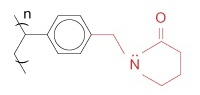
\includegraphics{Bilder/SPE_LCMS/mg_spe_strata-x.jpg}
    \caption{Sorbent polymer used for SPE, surface-modified styrene divinylbenzene.}
    \label{fig:StatPhase}
\end{figure}

\subsection{LC-MS/MS}
Liquid chromatography separates compounds in a mixture based on polarity by using a stationary phase that retards hydrophobic compounds while allowing more polar compounds to pass through faster along with the polar mobile phase. The compounds are then ionized by a strong voltage into fragment ions that are detected by a mass spectrometer that determines the mass of the transitions. Quantification of PFAS was determined by UPLC-MS/MS with an Acquity UPLC I-Class system connected to a Xevo TQ-S triple quadrupole mass spectrometer equipped with an ESI Z spray, both supplied by Waters (Milford, MA, USA). A Kinetex C18 column (30 x 2.1 mm, 1.3 \textmu m) serially connected to a Phenomenex C18 (2 x 2.1 mm i.d.) security guard (Torrance, CA, USA) was used for chromatographic separation. Mobile phases were A: 2 mM ammonium acetate in Milli-Q water (water phase) and B: pure MeOH (organic phase) that were supplied at a constant flow rate of 250 \textmu L min\textsuperscript{-1} to the LC column maintained at a temperature of 30 \textdegree C. The sample injection volume was 4 \textmu L. The run time for each sample was 6 minutes with an initial and final mobile phase gradient of 20:80 (A:B). Analytes were ionized by negative electrospray ionization (ESI-) and nitrogen was used as drying gas at the ionization source. Two ion transitions were monitored for each PFCA (\cref{tab:transitions}) within 60 s of the expected retention time for the compound. Peak integration was performed automatically by MassLynx software obtaining 12 points per peak and an average baseline peak width of 5 s. Data from UPLC-MS/MS was processed in MassLynx version 4.1 and quantification processing was performed with TargetLynx. Each peak was manually reviewed to remove marked peaks that were likely to be background noise and corrected for inconsistencies in peak width. Complete instrument programming and parameters are summarized in \cref{appSec:LCMS}.

\begin{table}
\centering
\caption{Ion transitions for the target analytes and internal standards in this study.}
\adjustbox{max width=\textwidth}{%
\begin{threeparttable}
\label{tab:transitions}
\begin{tabular}{ccccccl} \toprule
\textbf{Compound} &  \textbf{Structure} & \textbf{Formula} & \textbf{M} & \textbf{Parent} & \textbf{Cone (V)} & \textbf{Transitions (CE)}  \\ \midrule
& & & & & & \\
\multirow{2}{*}{PFPeA} &  \multirow{2}{*}{\chemfig[atom style={scale=0.5}]{O=[:90](-[:30,,,1]OH)-[:150](-[:112.5]F)(-[:67.5]F)-[:210](-[:292.5]F)(-[:247.5]F)-[:150](-[:112.5]F)(-[:67.5]F)-[:210](-[:270]F)(-[:150]F)-[:210]F}} & \multirow{2}{*}{$\mathrm{C_5HF_9O_2}$} & \multirow{2}{*}{264.05} & \multirow{2}{*}{262.97} & \multirow{2}{*}{20} & \multirow{2}{*}{262.97 $\rightarrow$ 219 (8)} \\
& & & & & & \\
& & & & & & \\
 &  &  &  &  &  &    \\
\multirow{2}{*}{PFHxA} &  \multirow{2}{*}{\chemfig[atom style={scale=0.5}]{O=[:90](-[:30,,,1]OH)-[:150](-[:112.5]F)(-[:67.5]F)-[:210](-[:292.5]F)(-[:247.5]F)-[:150](-[:112.5]F)(-[:67.5]F)-[:210](-[:292.5]F)(-[:247.5]F)-[:150](-[:210]F)(-[:150]F)-[:90]F}} & \multirow{2}{*}{$\mathrm{C_6HF_{11}O_2}$} & \multirow{2}{*}{314.05} & \multirow{2}{*}{312.97} & \multirow{2}{*}{10} & 312.97 $\rightarrow$ 118.95 (18) \\
 &  &  &  &  &  &   312.97 $\rightarrow$ 269 (8) \\
 & & & & & & \\
 & & & & & & \\
\multirow{2}{*}{PFHpA} &  \multirow{2}{*}{\chemfig[atom style={scale=0.5}]{O=[:90](-[:30,,,1]OH)-[:150](-[:67.5]F)(-[:112.5]F)-[:210](-[:247.5]F)(-[:292.5]F)-[:150](-[:67.5]F)(-[:112.5]F)-[:210](-[:247.5]F)(-[:292.5]F)-[:150](-[:67.5]F)(-[:112.5]F)-[:210](-[:150]F)(-[:210]F)-[:270]F}} & \multirow{2}{*}{$\mathrm{C_7HF_{13}O_2}$} & \multirow{2}{*}{364} & \multirow{2}{*}{362.96} & \multirow{2}{*}{6} & 362.96 $\rightarrow$ 119.00 (22) \\
 &  &  &  &  &  &   362.96 $\rightarrow$ 168.97 (18) \\
 & & & & & & \\
 & & & & & & \\
\multirow{2}{*}{PFOA} &  \multirow{2}{*}{\chemfig[atom style={scale=0.5}]{O=[:90](-[:30,,,1]OH)-[:150](-[:67.5]F)(-[:112.5]F)-[:210](-[:247.5]F)(-[:292.5]F)-[:150](-[:67.5]F)(-[:112.5]F)-[:210](-[:247.5]F)(-[:292.5]F)-[:150](-[:67.5]F)(-[:112.5]F)-[:210](-[:247.5]F)(-[:292.5]F)-[:150](-[:90]F)(-[:150]F)-[:210]F}} & \multirow{2}{*}{$\mathrm{C_8HF_{15}O_2}$} & \multirow{2}{*}{414.07} & \multirow{2}{*}{412.97} & \multirow{2}{*}{20} & 412.97 $\rightarrow$ 168.90 (18) \\
 &  &  &  &  &    & 412.97 $\rightarrow$ 369.00 (8) \\
 & & & & & & \\
 & & & & & & \\
\multirow{2}{*}{PFNA} &  \multirow{2}{*}{\chemfig[atom style={scale=0.5}]{O=[:90](-[:30,,,1]OH)-[:150](-[:112.5]F)(-[:67.5]F)-[:210](-[:292.5]F)(-[:247.5]F)-[:150](-[:112.5]F)(-[:67.5]F)-[:210](-[:292.5])(-[:247.5]F)-[:150](-[:112.5]F)(-[:67.5]F)-[:210](-[:292.5]F)(-[:247.5]F)-[:150](-[:112.5]F)(-[:67.5]F)-[:210](-[:270]F)(-[:210]F)-[:150]F}} & \multirow{2}{*}{$\mathrm{C_9HF_{17}O_2}$} & \multirow{2}{*}{464.08} & \multirow{2}{*}{462.99} & \multirow{2}{*}{20} & 462.99 $\rightarrow$ 219 (16) \\
 &  &  &  &  &    & 462.99 $\rightarrow$ 419 (10) \\
  & & & & & & \\
  & & & & & & \\
\multirow{2}{*}{PFDA} &  \multirow{2}{*}{\chemfig[atom style={scale=0.5}]{O=[:90](-[:30,,,1]OH)-[:150](-[:112.5]F)(-[:67.5]F)-[:210](-[:292.5]F)(-[:247.5]F)-[:150](-[:112.5]F)(-[:67.5]F)-[:210](-[:292.5]F)(-[:247.5]F)-[:150](-[:112.5]F)(-[:67.5]F)-[:210](-[:292.5]F)(-[:247.5]F)-[:150](-[:112.5]F)(-[:67.5]F)-[:210](-[:292.5]F)(-[:247.5]F)-[:150](-[:210]F)(-[:150]F)-[:90]F}} & \multirow{2}{*}{$\mathrm{C_{10}HF_{19}O_2}$} & \multirow{2}{*}{514.09} & \multirow{2}{*}{513.1} & \multirow{2}{*}{10} & 513.10 $\rightarrow$ 219.01 (18) \\
 &  &  &  &  &    & 513.10 $\rightarrow$ 269.04 (16) \\ 
 & & & & & & \\
 & & & & & & \\ \midrule
 \multicolumn{7}{c}{\textit{Internal standards (IS)}} \\ \midrule
  & & & & & & \\
 \multirow{2}{*}{PFOA \textsuperscript{13}C\textsubscript{8}} & \multirow{2}{*}{\chemfig[atom style={scale=0.5}]{O=[:90](-[:30,,,1]OH)-[:150](-[:67.5]F)(-[:112.5]F)-[:210](-[:247.5]F)(-[:292.5]F)-[:150](-[:67.5]F)(-[:112.5]F)-[:210](-[:247.5]F)(-[:292.5]F)-[:150](-[:67.5]F)(-[:112.5]F)-[:210](-[:247.5]F)(-[:292.5]F)-[:150](-[:90]F)(-[:150]F)-[:210]F}} & \multirow{2}{*}{$\mathrm{^{13}C_8HF_{15}O_2}$} & \multirow{2}{*}{422.01} & \multirow{2}{*}{420.9} & \multirow{2}{*}{16} & 420.90 $\rightarrow$ 171.86 (16) \\
 &  &  &  &  &    & 420.90 $\rightarrow$ 222.84 (16) \\ 
 & & & & & & \\
 & & & & & & \\
  \multirow{2}{*}{PFOS \textsuperscript{13}C\textsubscript{8}} & \multirow{2}{*}{\chemfig[atom style={scale=0.5}]{F-[:67.5](-[:292.5]F)(-[:30]S(=[:300]O)(-[:30,,,1]OH)=[:120]O)-[:150](-[:67.5]F)(-[:112.5]F)-[:210](-[:247.5]F)(-[:292.5]F)-[:150](-[:67.5]F)(-[:112.5]F)-[:210](-[:247.5]F)(-[:292.5]F)-[:150](-[:67.5]F)(-[:112.5]F)-[:210](-[:247.5]F)(-[:292.5]F)-[:150](-[:90]F)(-[:150]F)-[:210]F}} & \multirow{2}{*}{$\mathrm{^{13}C_8HF_{17}O_3}S$} & \multirow{2}{*}{507.06} & \multirow{2}{*}{506.9} & \multirow{2}{*}{56} & 506.90 $\rightarrow$ 79.87 (46) \\
 &  &  &  &  &    & 506.90 $\rightarrow$ 171.85 (32) \\ 
 & & & & & & \\
 & & & & & & \\ 
 \multirow{2}{*}{6:2 FTS \textsuperscript{13}C\textsubscript{2}} & \multirow{2}{*}{\chemfig[atom style={scale=0.5}]{O=[:60]S(=[:60]O)(-[:330,,,1]OH)-[:150]-[:210]-[:150](-[:67.5]F)(-[:112.5]F)-[:210](-[:247.5]F)(-[:292.5]F)-[:150](-[:67.5]F)(-[:112.5]F)-[:210](-[:247.5]F)(-[:292.5]F)-[:150](-[:67.5]F)(-[:112.5]F)-[:210](-[:270]F)(-[:210]F)-[:150]F}} & \multirow{2}{*}{$\mathrm{C_{6}^{13}C_2H_{5}F_{13}O_3S}$} & \multirow{2}{*}{432} & \multirow{2}{*}{432.96} & \multirow{2}{*}{26} & 432.96 $\rightarrow$ 411.959 (24) \\
 &  &  &  &  &    & 432.96 $\rightarrow$ 81.901 (30) \\ 
 & & & & & & \\
 & & & & & & \\ \bottomrule
\end{tabular}
\begin{tablenotes}
\item CE = capillary electrophoresis
\end{tablenotes}
\end{threeparttable}}
\end{table}

\subsection{Quality assurance and quality control}
The analytical validity of SPE and LC-MS/MS were assured by preparing a set of QA/QC samples. An overview of the concentrations, contents and addition of analytes in the quality controls are in \cref{tab:QC}.

\subsubsection{Blanks}
Contamination that may arise during preparation of samples and from laboratory materials was evaluated through the analysis of sample and procedural blanks. One procedural blank was prepared by spiking IS directly into the cartridge and eluting with methanol, continuing SPE from this point. Contamination from test tubes, reagents or other introductions of contamination will show up on the instrument results from this QA. Two blank samples were prepared by bringing 50 mL pH 3 MQ water (sample matrix) spiked with IS through the extraction protocol. Sample blanks determine any interferences caused by the the matrix itself. During analysis, solvent blanks (100 \% MeOH) and a standard mixture of TAs at 10 ppb were injected every 15-20 samples to monitor potential cross contamination, carryover, and assuring maintenance of sensitivity. A MeOH:Milli-Q (50:50; v/v) 0.1 \% formic acid wash solution was used to clean the injection needle before and after each injection.

\subsubsection{Pre- and post- extraction spiked matrix samples}
QA/QC pre- and post-extraction matrix spike samples were prepared in triplicates at a concentration interval covering the expected concentration range of the test samples (2.5, 25 and 50 ppb). A working standard of target analytes (C5-C10) was prepared at 1 ppm in MeOH for spiking the samples. Pre-extraction matrix spikes were prepared by spiking IS and TA standard at 2.5, 25 and 50 ppb in 50 mL sample matrix. These were taken through the protocol in the same manner as the test samples. Matrix matched samples were prepared by taking 50 mL sample matrix through the SPE protocol and spiking with 2.5, 25 and 50 ppb TA and IS post-extraction. 

\subsubsection{Absolute recovery, relative recovery and matrix effect calculations}
Recovery (R), relative recovery (RR) and matrix effects (ME) were calculated for each TA by comparing the pre- and post-extraction matrix spike signals. R and RR were assessed by the the following equations:

\begin{equation}
    \label{eq:Recovery}
    \mathrm{\% AR  = 100 \% \times \left ( \frac{A_{ss}}{A_{se}} \right ) }
\end{equation}

\begin{equation}
    \label{eq:relativeRecovery}
    \mathrm{\% RR = \frac{\frac{A_{ss}}{A_{is}}-\frac{A_{b}}{A_{is}}}{\frac{A_{se}}{A_{is}}-\frac{A_{b}}{A_{is}}}\times 100 \% }
\end{equation}

where 100 \% indicates recovery of all analytes. Matrix effects is assessed by the following equation:

\begin{equation}
    \label{eq:ME}
    \mathrm{\% ME = 100 \% \times \left(\frac{A_{se} - A_b}{A_{cc}}\right )-1 }
\end{equation}

where ME \textgreater 0\% indicates ion enhancement, and ME \textless 0\% = ion suppression. Matrix effects (MEs, \%) during measurements were assessed and estimated as X, X, X, X, X, X for PFPeA, PFHxA, PFHpA, PFOA, PFNA, and PFDA, respectively.

Where: \newline
\newline
\begin{tabular}{p{1cm}p{20cm}}
    \textit{A}   & peak area of chromatogram signal, \\
    \textit{ss}  & spiked sample (pre-extraction matrix spike), \\
    \textit{se}  & spiked extract (post-extraction matrix matched), \\
    \textit{is}  & internal standard, \\
    \textit{b}   & solvent blank, \\
    \textit{cc}  & calibration curve solvent spike \\
\end{tabular} \\

\subsubsection{Calibration curves}
A 10-point calibration curve ranging from 0.01 to 50 ppb was prepared in methanol. The results demonstrated a satisfactory regression coefficient ($R^2$ \textgreater 0.98) for each analyte. This solvent blank calibration curve is used to derive analyte concentrations in samples not taken through the SPE protocol since they do not  A calibration curve that accounts for matrix effect is made by comparing the matrix matched samples to the calibration curve solvent spikes.

During calculations of results, only \textsuperscript{13}C\textsubscript{8}-PFOA was used because it had the most similar retention time as the target analytes. 

\begin{table}
\caption{Quality assurance and quality controls.}
\centering
\adjustbox{max width=\textwidth}{%
\begin{threeparttable}
\label{tab:QC}
\begin{tabular}{lcccccc}
\toprule
\multicolumn{1}{c}{\textbf{Code}} & \textbf{\begin{tabular}[c]{@{}c@{}}Sample \\ matrix\end{tabular}} & \textbf{\begin{tabular}[c]{@{}c@{}}TA (addition \\ pre-extraction)\end{tabular}} & \textbf{\begin{tabular}[c]{@{}c@{}}IS (addition \\ pre-extraction)\end{tabular}} & \textbf{\begin{tabular}[c]{@{}c@{}}TA (addition \\ post-extraction)\end{tabular}} & \textbf{\begin{tabular}[c]{@{}c@{}}IS (addition\\  post-extraction\end{tabular}} & \multicolumn{1}{c}{\textbf{\begin{tabular}[c]{@{}c@{}}Solvent\\ (MQ:MeOH)\end{tabular}}} \\ \midrule
Procedural blank & NO &  & \checkmark &  & & 50:50 \\ \hline
Blank 1 & YES &  & \checkmark &  & & 50:50 \\ 
Blank 2 & YES &  & \checkmark &  & & 50:50 \\ \hline
Spike 2.5 ppb & YES & \checkmark & \checkmark &  & & 50:50 \\ 
Spike 25 ppb & YES & \checkmark & \checkmark &  & & 50:50 \\ 
Spike 50 ppb & YES & \checkmark & \checkmark &  &  & 50:50\\ \hline
Matrix matched 2.5 ppb & YES &  &  & \checkmark & \checkmark & 50:50\\
Matrix matched 25 ppb & YES &  &  & \checkmark & \checkmark & 50:50\\
Matrix matched 50 ppb & YES &  &  & \checkmark & \checkmark & 50:50\\ \hline
Solvent blank\tnote{*} & NO & & & & & 0:100\\
Calibration 0 ppb & NO &  &  & \checkmark & \checkmark & 0:100 \\ 
Calibration 0.01 ppb & NO&  &  & \checkmark & \checkmark & 0:100\\
Calibration 0.05 ppb & NO&  &  & \checkmark & \checkmark & 0:100\\
Calibration 0.1 ppb & NO&  &  & \checkmark & \checkmark & 0:100\\
Calibration 0.2 ppb & NO&  &  & \checkmark & \checkmark & 0:100\\
Calibration 0.5 ppb & NO&  &  & \checkmark & \checkmark & 0:100\\
Calibration 1 ppb & NO&  &  & \checkmark & \checkmark & 0:100\\
Calibration 2 ppb & NO&  &  & \checkmark & \checkmark & 0:100\\
Calibration 5 ppb & NO&  &  & \checkmark & \checkmark & 0:100\\
Calibration 10 ppb\tnote{*} & NO &  &  & \checkmark & \checkmark & 0:100\\
Calibration 25 ppb & NO&  &  & \checkmark & \checkmark & 0:100\\
Calibration 50 ppb & NO&  &  & \checkmark & \checkmark & 0:100\\ \bottomrule
\end{tabular}
\begin{tablenotes}
\item[*] Injected every 15-20 samples
\item TA = target analytes, IS = internal standard
\end{tablenotes}
\end{threeparttable}}
\end{table} %table with quality control parameters

%%%%%%%%%%%%%%%%%%%%%%%%%%%%%%%%%%%%%%%%%%%%%%%%%%%%%%%%%%%%%%%%%%%%%%%%%%%%%%%%%%%%%%%%%%%%%%%%%%%%%%%%%%%%%%%%%%%%%%%%%%%
\section{Supporting parameters/sorbent characterization}

\subsection{Iron oxide characterization}
Synchrotron iron oxide characterization Gabrielle.
The digested sludge Lindum and Ullensaker sludge biochars were submitted to the synchrotron for iron oxide speciation. The biochars were crushed in a mortar and sieved to \textless 250 \textmu m fine powder until no visible particles were present. Next, boron nitride (BN) was added to the powdered biochar mixed with a mortar and scraped from the sides with a spatula, repeated ten times to a homogeneous powder. Then transferred to LC vials that were taken to the ESRF Synchrotron. The powder was pressed into pellets and submitted to the beam.

The synchrotron analysis was performed in France

\subsection{Surface area and porosity}
University of Florida, CO\textsubscript{2} and N\textsubscript{2} sorptometry. 

\subsection{Elemental composition}
Total C, H, O, N, P content


%%%%%%%%%%%%%%%%%%%%%%%%%%%%%%%%%%%%%%%%%%%%%%%%%%%%%%%%%%%%%%%%%%%%%%%%%%%%%%%%%%%%%%%%%%%%%%%%%%%%%%%%%%%%%%%%%%%%%%%%%%%

\section{Data analysis}
Peak integration: 
Statistical analysis software: R and Excel for simple statistical analyses and organization. 

